%%%%%%%%%%%%%%%%%%%%%%%%%%%%%%%%%%%%%%%%%%%%%%%%%%%%%%%
%%%%               FORMATTING AND COLORING         %%%%
%%%%%%%%%%%%%%%%%%%%%%%%%%%%%%%%%%%%%%%%%%%%%%%%%%%%%%%
\documentclass[xcolor=dvipsnames]{beamer}

\definecolor{Fuchsia}{HTML}{49796b}
\definecolor{SlateGrey}{HTML}{003800}
\definecolor{FuchsiaDark}{HTML}{305047}

%\definecolor{LightGrey}{HTML}{666666}

\colorlet{accent}{Fuchsia}
\colorlet{emphasis}{SlateGrey}

\usepackage{caption}

\usetheme{CambridgeUS}
\useinnertheme{rectangles}
\useoutertheme{infolines}

%%%%%%%%%%%%%%%%%%%%%%%%%%%%%%%%%%%%%%%%%%%%%
%this adds in the circles to the right of background
%%%%%%%%%%%%%%%%%%%%%%%%%%%%%%%%%%%%%%%%%%%%%
\makeatletter
\def\insertsubsectionnavigationhorizontal#1#2#3{%
    \hbox to #1{{%
        \usebeamerfont{subsection in head/foot}\usebeamercolor[fg]{subsection in head/foot}
        \beamer@currentsubsection=0%
        \def\sectionentry##1##2##3##4##5{}%
        \def\slideentry##1##2##3##4##5##6{\ifnum##6=\c@part\ifnum##1=\c@section%
      \ifnum##2>\beamer@currentsubsection%
      \box\beamer@sectionbox\hskip1.875ex plus1fill%
            \hbox to 0pt{%
                    \global\beamer@section@min@dim\beamer@tempdim
                        \beamer@link(##4){%
                            \usebeamerfont{mini frame}%
                            \ifnum\c@section=##1%
                                \ifnum\c@subsection=##2%
                                    \usebeamercolor[fg]{mini frame}%
                                    \ifnum\c@subsectionslide=##3%
                                        \usebeamertemplate{mini frame}%\beamer@minislidehilight%
                                    \else%
                                        \usebeamertemplate{mini frame in current subsection}%\beamer@minisliderowhilight%
                                    \fi%
                                \else%
                                    \usebeamercolor{mini frame}%
                                    %\color{fg!50!bg}%
                                    \usebeamertemplate{mini frame in other subsection}%\beamer@minislide%
                                \fi%
                            \else%
                                \usebeamercolor{mini frame}%
                                                                %\color{fg!50!bg}%
                                \usebeamertemplate{mini frame in other subsection}%\beamer@minislide%
                            \fi%
                        }%
                \hskip-10cm plus 1fil%
            }%
            \fi\fi\fi\ignorespaces
        }%
        #2\hskip.3cm\setbox\beamer@sectionbox=\hbox{}%
        \hskip-1.875ex plus-1fill\dohead%
        \box\beamer@sectionbox\hfil\hskip.3cm%
        #3
    }}
}

\setbeamertemplate{footline}%{infolines theme}
{
  \leavevmode%
  \hbox{%
  \begin{beamercolorbox}[wd=.333333\paperwidth,ht=2.25ex,dp=1ex,center]{author in head/foot}%
    \usebeamerfont{author in head/foot}\insertshortauthor\expandafter\beamer@ifempty\expandafter{\beamer@shortinstitute}{}{~~(\insertshortinstitute)}
  \end{beamercolorbox}%
  \begin{beamercolorbox}[wd=.333333\paperwidth,ht=2.25ex,dp=1ex,center]{title in head/foot}%
    \usebeamerfont{title in head/foot}\insertshorttitle
  \end{beamercolorbox}%
  \begin{beamercolorbox}[wd=.333333\paperwidth,ht=2.25ex,dp=1ex,right]{date in head/foot}%
    \usebeamerfont{date in head/foot} %\insertshortdate{} % remove the date from each slide 
    % could insert text here to make it display in the footer 
    \hspace*{2em}
    \insertframenumber{} / \inserttotalframenumber\hspace*{2ex} 
  \end{beamercolorbox}}%
  \vskip0pt%
}
\makeatother

\setbeamertemplate{headline}
{
  \leavevmode%
  \hbox{%
  \begin{beamercolorbox}[wd=.5\paperwidth,ht=2.65ex,dp=1.5ex,right]{section in head/foot}%
    \usebeamerfont{section in head/foot}\bfseries\insertsectionhead\hspace*{2ex}
  \end{beamercolorbox}%
  \begin{beamercolorbox}[wd=.5\paperwidth,ht=2.65ex,dp=1.5ex,left]{subsection in head/foot}%
    \usebeamerfont{subsection in head/foot}\setbeamercolor{section in head/foot}{fg=Fuchsia!125,bg=white}
    \vspace*{.01cm}\insertsubsectionnavigationhorizontal{.5cm}{\hskip-.1cm}{}
  \end{beamercolorbox}}%
  \vskip0pt%
}
% gets rid of navigation symbols
\setbeamertemplate{navigation symbols}{}
% add figures numbering
\setbeamertemplate{caption}[numbered]

\setbeamercolor{frametitle}{fg=Fuchsia,bg=Fuchsia!20}
\setbeamercolor{section in head/foot}{fg= SlateGrey!20, bg=Fuchsia}
\setbeamercolor{title in head/foot}{fg=Fuchsia}
\setbeamercolor{subsection in head/foot}{fg=Fuchsia}
\setbeamercolor{author in head/foot}{bg=Fuchsia, fg=Fuchsia}
\setbeamercolor{date in head/foot}{fg=Fuchsia}
\setbeamercolor{structure}{fg=Fuchsia, bg= SlateGrey}
\setbeamercolor{frametitle}{fg= Fuchsia}
\setbeamercolor{title}{fg=Fuchsia}
\setbeamercolor*{palette tertiary}{bg=Fuchsia}
\setbeamercolor{section in sidebar}{fg=Fuchsia}
\setbeamercolor{titlelike}{bg =SlateGrey!5}

%%%%%%%%%%%%%%%%%%%%%%%%%%%%%%%%%%%%%%%%%%%%%%%%%%%
% End of customizing the theme layout and colors 
%%%%%%%%%%%%%%%%%%%%%%%%%%%%%%%%%%%%%%%%%%%%%%%%%%%
\usepackage{comment}
\usepackage[T1]{fontenc}
\usepackage[default]{lato}
\usepackage[english]{babel}
\usepackage[utf8x]{inputenc}
\usepackage{pslatex}
\usepackage{fontawesome}
\usepackage{animate}

\usepackage{xmpmulti}

\usepackage{subcaption}
\captionsetup{compatibility=false}
%%%%%%%%%%%%%%%%%%%%%%%%%%%%%%%%%%%%%%%%%%%%%%%%%%%%%%%
%%%%%%%%%%%%%%%%%%%%%%%%%%%%%%%%%%%%%%%%%%%%%%%%%%%%%%%
%%%%          Beginning of the slide deck          %%%%
%%%%%%%%%%%%%%%%%%%%%%%%%%%%%%%%%%%%%%%%%%%%%%%%%%%%%%%
%%%%%%%%%%%%%%%%%%%%%%%%%%%%%%%%%%%%%%%%%%%%%%%%%%%%%%%

\definecolor{climateChange}{HTML}{F8766D}
\definecolor{recentTrends}{HTML}{00BFC4}
\definecolor{activeGreen}{HTML}{00cc00}
\definecolor{fuelBreakColor}{HTML}{70AD47}
\definecolor{salvageLogColor}{HTML}{0099FF}
\definecolor{fuelReductionColor}{HTML}{EB45BC}


\newenvironment{a2env}{\only{\setbeamercolor{local structure}{fg=climateChange}}}{}
\newenvironment{rtenv}{\only{\setbeamercolor{local structure}{fg=recentTrends}}}{}
%%%%%%%%%%%%
%title page%
%%%%%%%%%%%%
\title[Harvard Forest REU Symposium]{Simulating effects of forest management practices in a fire prone region of the Northwestern US}
\author{Evan Waldmann}
\institute{University of Central Florida}
\date{\scriptsize{August 2nd, 2018}}

\begin{document}
\begin{frame}
  \titlepage
  \vfill
  
\includegraphics[width=.1\linewidth]{University-of-Central-Florida-logo-Black.png} \hfill 
\includegraphics[width=.11\linewidth]{Harvard_Forest_logo_high_res.jpg}
\end{frame}

\section{Background}


% Uncomment these lines for an automatically generated outline.
%\begin{frame}{Outline}
%  \tableofcontents
%\end{frame}


%%%%%%%%%%%%%%%%%%%%%%%%%%%
%beginning of actual sides%
%%%%%%%%%%%%%%%%%%%%%%%%%%%
\subsection{}


\section{Background}
\subsection{}

\begin{frame}{Objective of the Project}

\centering{ To model and simulate \textbf{dynamic} human response to forest disturbances in order to see the impacts that humans have on the landscape}

\end{frame}


\begin{frame}{Study Area: Klamath National Forest}
%\centering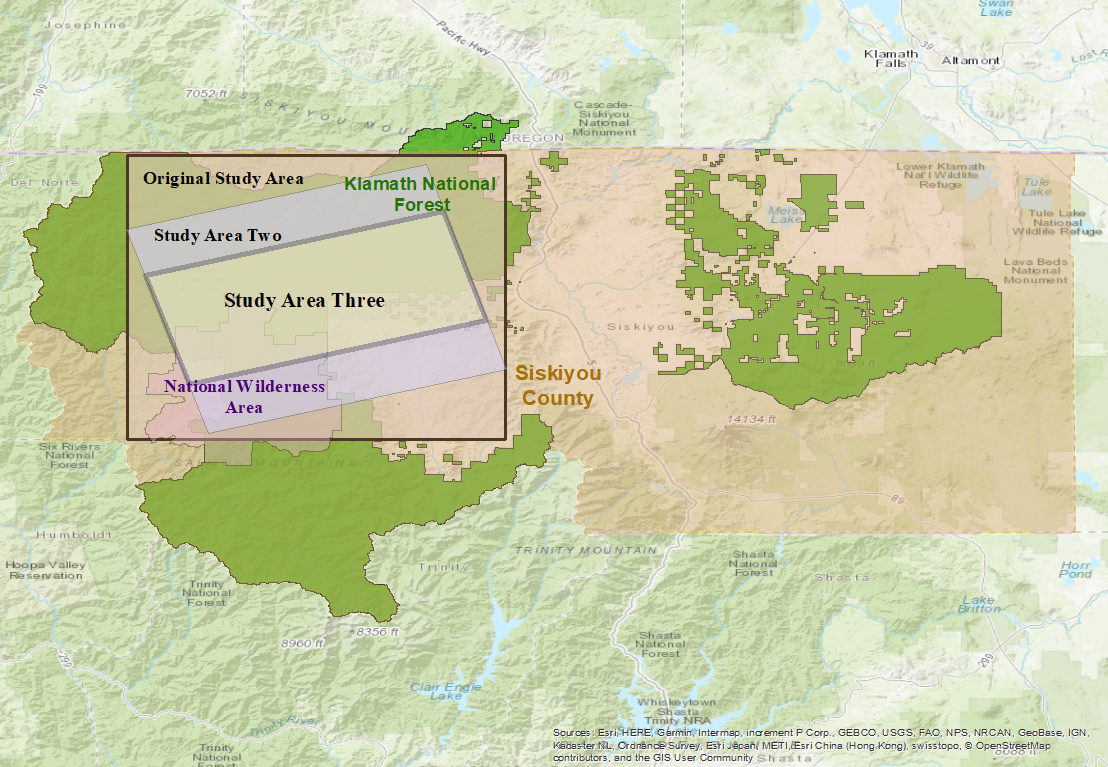
\includegraphics[width=.9\linewidth]{studyAreaMapNew.png}
%dimensions  : 101, 205, 20705  (nrow, ncol, ncell)
%resolution  : 270, 270  (x, y)
%extent      : -2234904, -2179554, 2378951, 2406221  (xmin, xmax, ymin, ymax)
%coord. ref. : +proj=aea +lat_1=29.5 +lat_2=45.5 +lat_0=23 +lon_0=-96 +x_0=0 +y_0=0 +datum=NAD83 +units=m +no_defs +ellps=GRS80 +towgs84=0,0,0 
\centering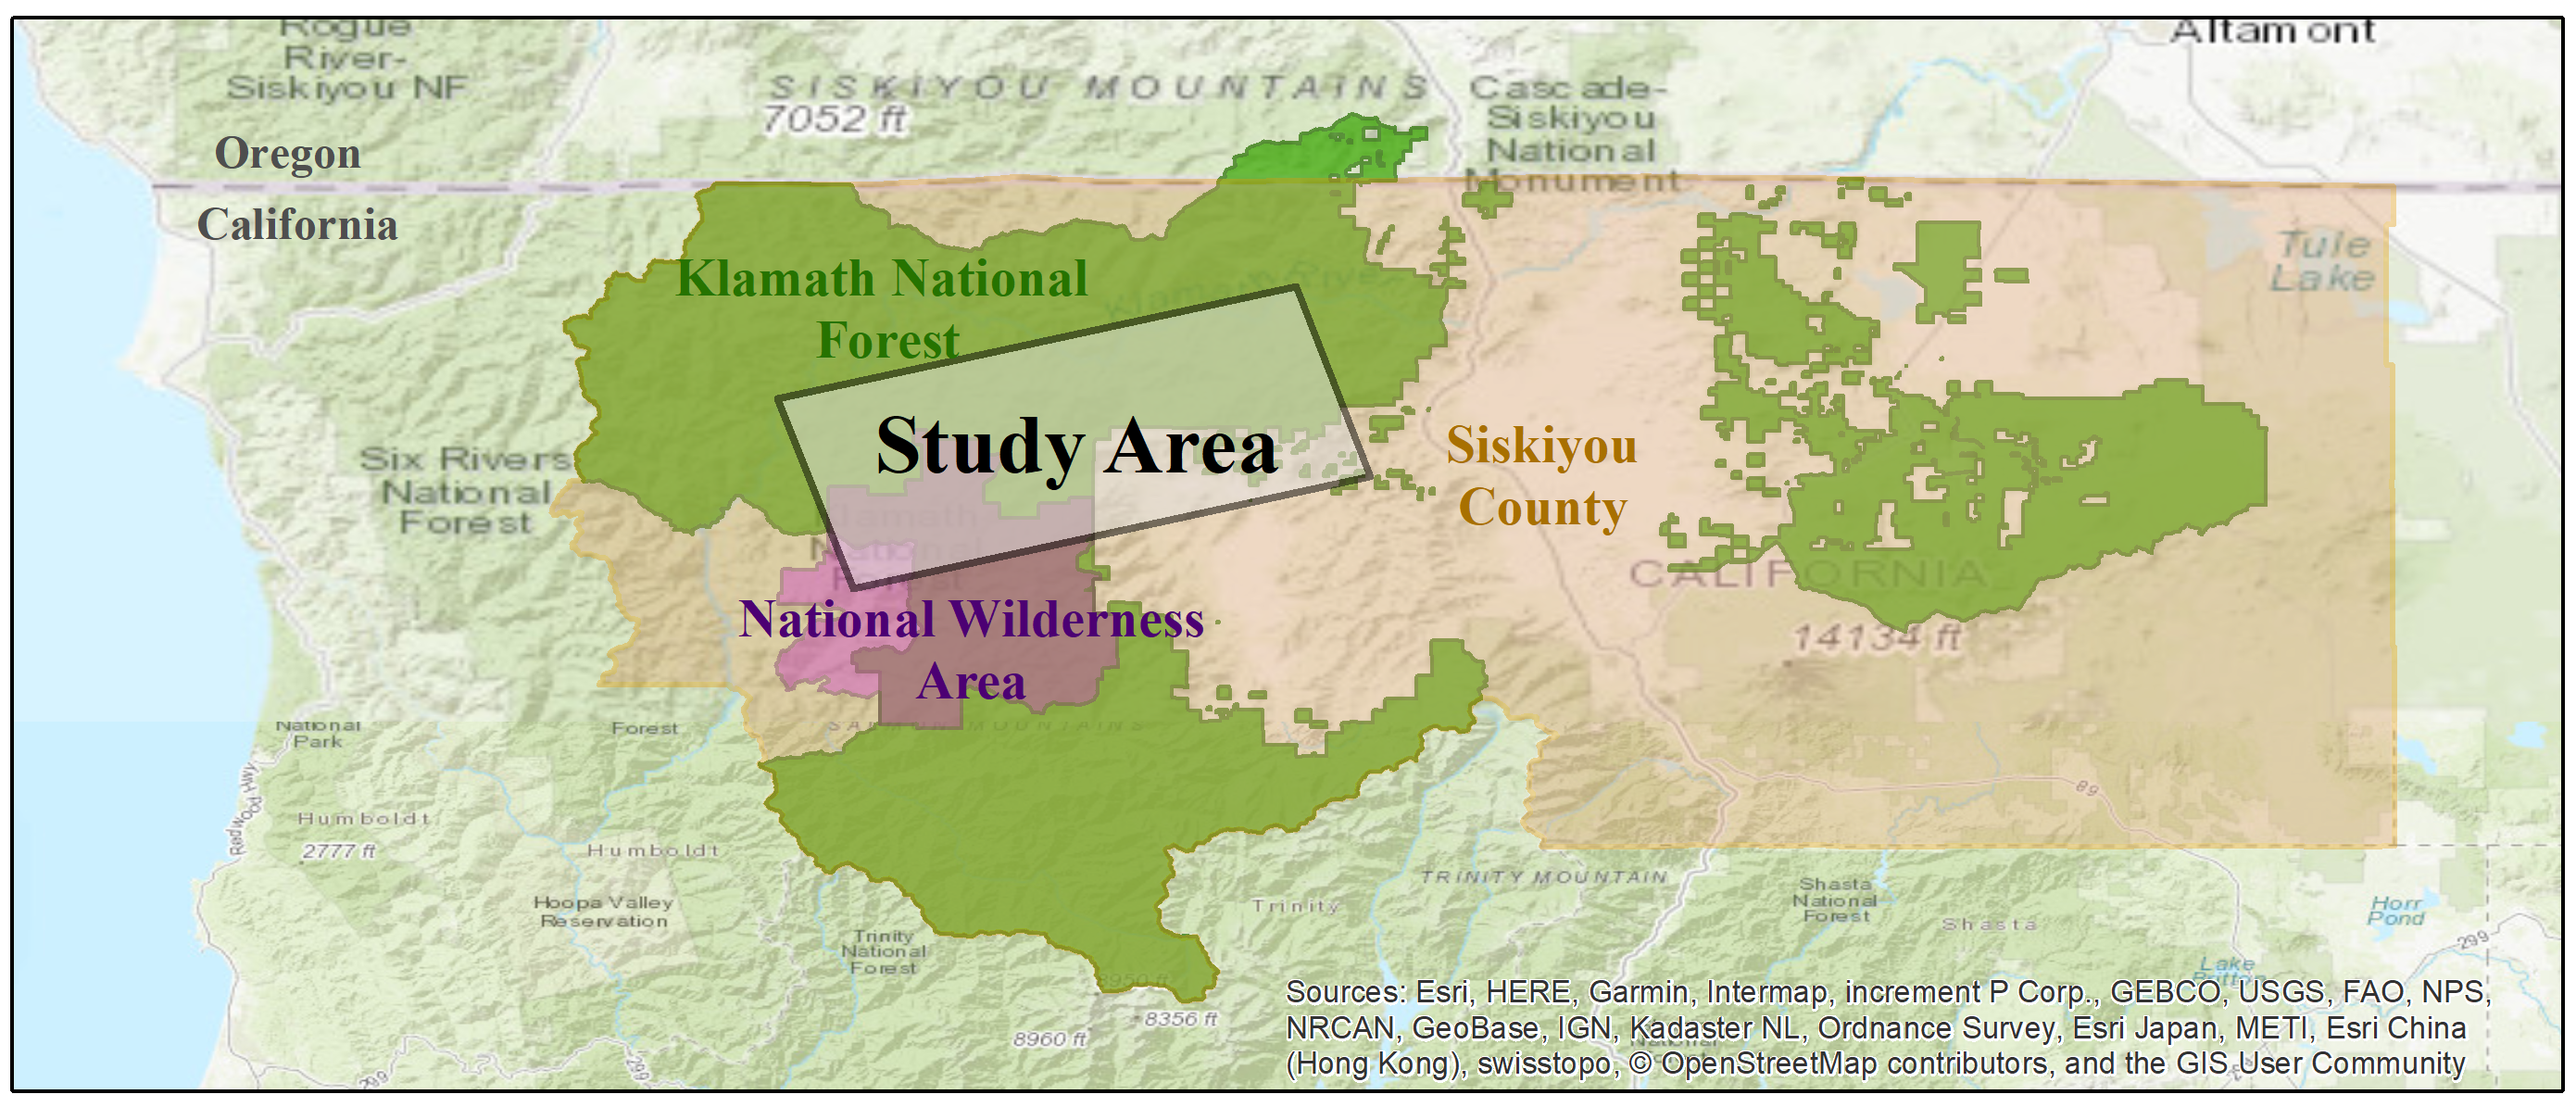
\includegraphics[width=.9\linewidth]{studyAreaThreeMap.png}

\vspace*{.1in}

\centering\begin{itemize}
\item[] Dimensions: 101 rows X 205 columns 
\item[] Cell resolution: 270m x 270m 
\item[] Size: 20,705 cells (138,043ha or 1,380km$^2$)
\item[] Timescale: 90 years (2010-2100) using 10 year time step
\end{itemize}
\end{frame}

\begin{frame}{Recent Headlines about the Klamath Region}
\begin{itemize}
\item \textbf{July 19, 2018} - Natchez Fire crosses into Klamath National Forest; burned an estimated \textbf{767} acres \textit{(NBC52)}
\item \textbf{July \textup{  } 9, 2018} - Klamathon Fire update; now at \textbf{35,250} acres, 30\% contained, 81 structures lost \textit{(Harald and News)} 
\item \textbf{June 28, 2018} - Cherry Fire: \textbf{100 }acre fire burning through vegetation near Horse Creek \textit{(News10)}
\end{itemize}



\begin{center}

\begin{columns}
    \begin{column}{0.4\textwidth}
\begin{figure}
\centering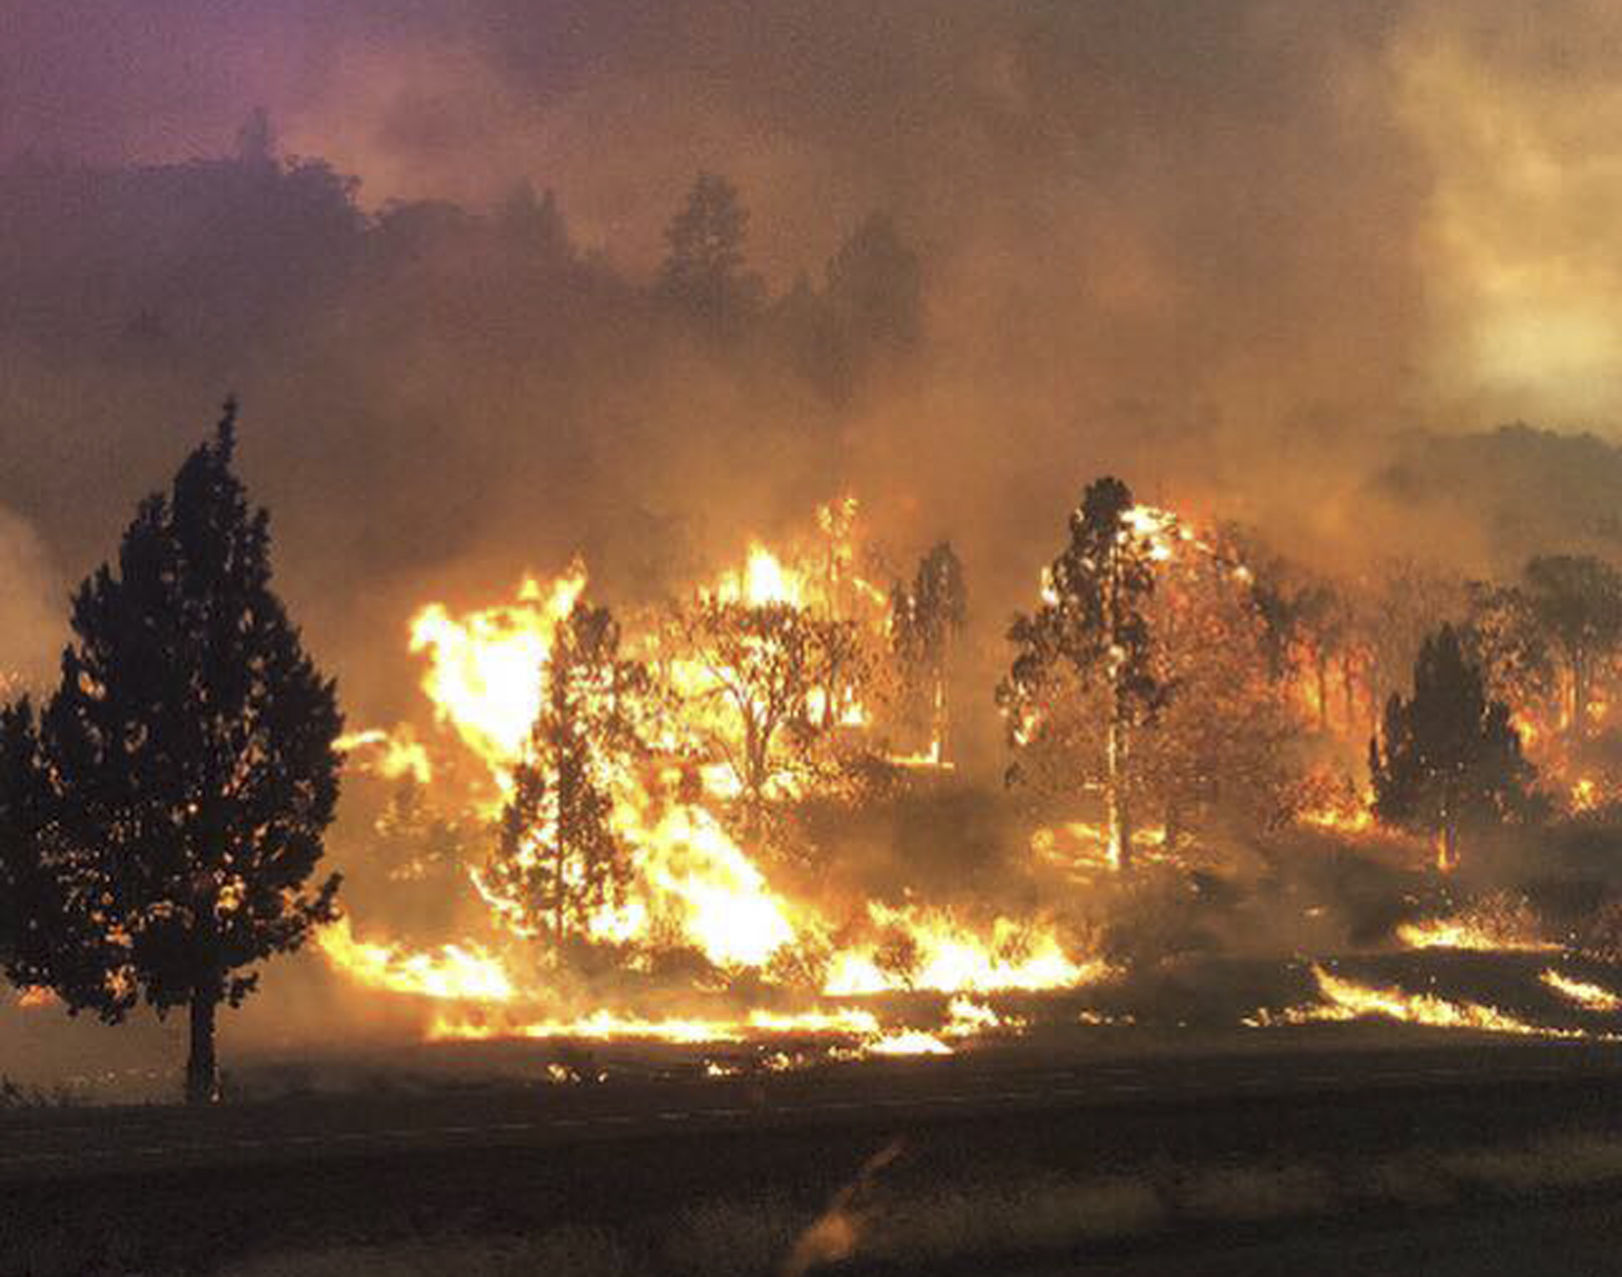
\includegraphics[width=.85\linewidth]{klamathFire_herald_and_news.jpg}
\caption*{{\hspace*{1.3cm}Klamathon Fire} \newline \tiny\textit{\hspace*{1.25cm}Photo from Harald and News}}
\end{figure}
    \end{column}
    \begin{column}{0.6\textwidth}
  \begin{figure}
\vspace*{-.5cm}
\centering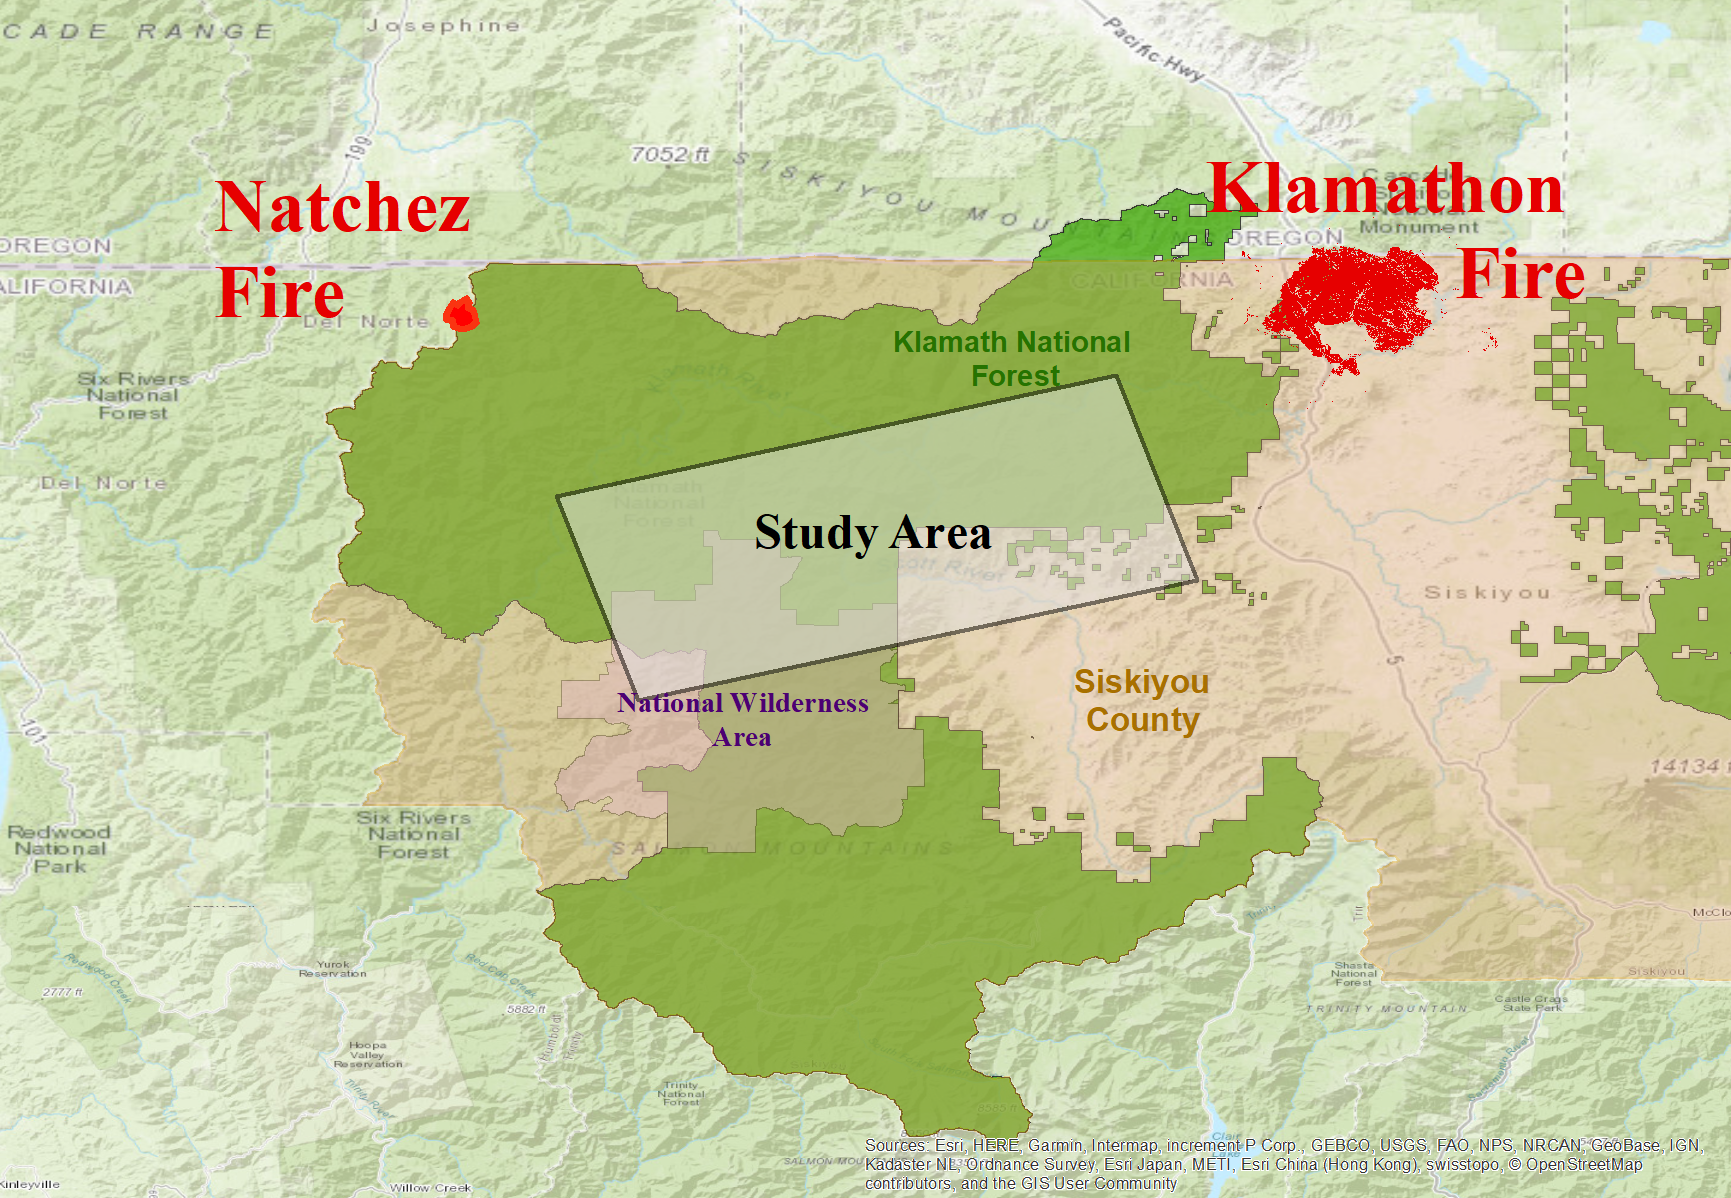
\includegraphics[width=.85\linewidth]{firemap2.png}

\end{figure}
    \end{column}
\end{columns}
\end{center}

\end{frame}



\begin{frame}{Experimental Design}

\begin{center}
\resizebox{\linewidth}{!}{
 \begin{tabular}{||l | l  c  c||} 
 \hline
Scenarios & Climate & Fire & Human Response \\ [0.5ex] 
 \hline\hline
 Historic Climate & \color{recentTrends}Historic Climate & Inactive & Inactive \\ 
 \hline
 Historic Climate \& Fire  & \color{recentTrends}Historic Climate & \color{activeGreen}Active & Inactive \\
 \hline
 Historic Climate \& LU & \color{recentTrends}Historic Climate & \color{activeGreen}Active & \color{activeGreen}Active \\
 \hline
 Climate Change & \color{climateChange}Climate Change & Inactive & Inactive \\
 \hline
 Climate Change \& Fire & \color{climateChange}Climate Change & \color{activeGreen}Active & Inactive \\ 
 \hline
 Climate Change \& LU  & \color{climateChange}Climate Change & \color{activeGreen}Active & \color{activeGreen}Active \\ 
 \hline
\end{tabular}}
\end{center}
\end{frame}


\begin{frame}{LANDIS-II}
 \centering LANDIS-II is a spatially explicit model that simulates forest growth and disturbances across landscapes.

\vfill

\centering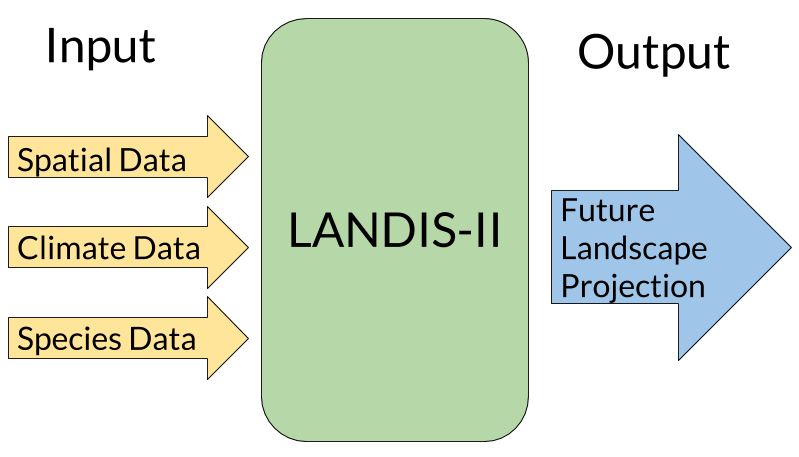
\includegraphics[width=.8\linewidth]{landis_basic.png}
\end{frame}


\begin{frame}{LANDIS-II Diagram}

\centering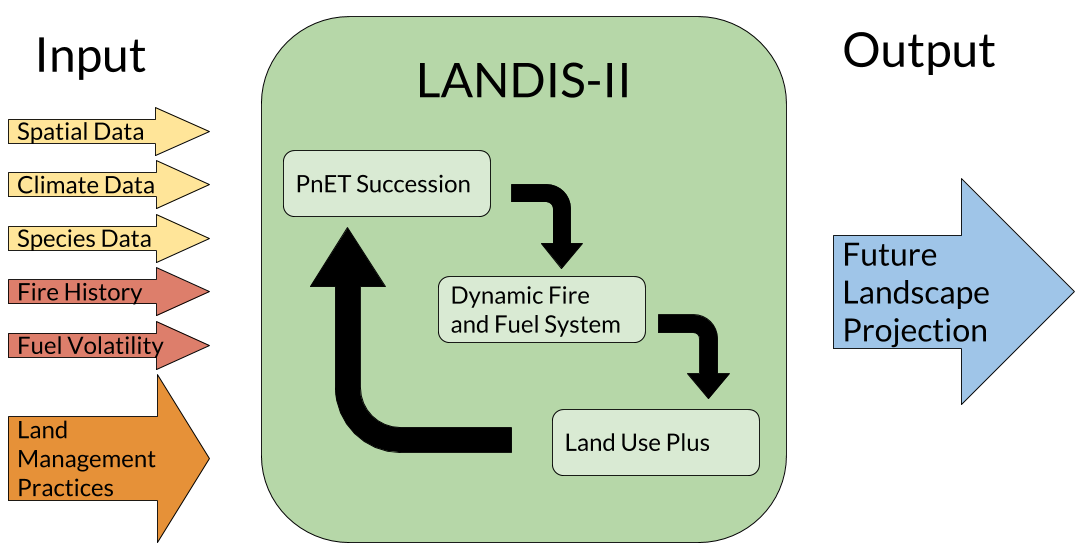
\includegraphics[width=\linewidth]{landis_complicated.png}

% Using a 10 year time step,
% \begin{itemize}
% \item forest growth was simulated with the \textbf{PnET-Succession (Photosynthesis and EvapoTranspiration) Extension},
% \item disturbances to the forest were simulated using the \textbf{Dynamic Fire and Fuels Extension}, and 
% \item human reaction to those disturbances were simulated with the \textbf{Land Use Plus Extension}.
% \end{itemize}
\end{frame}




\begin{frame}{What Existed and What I added}
\centering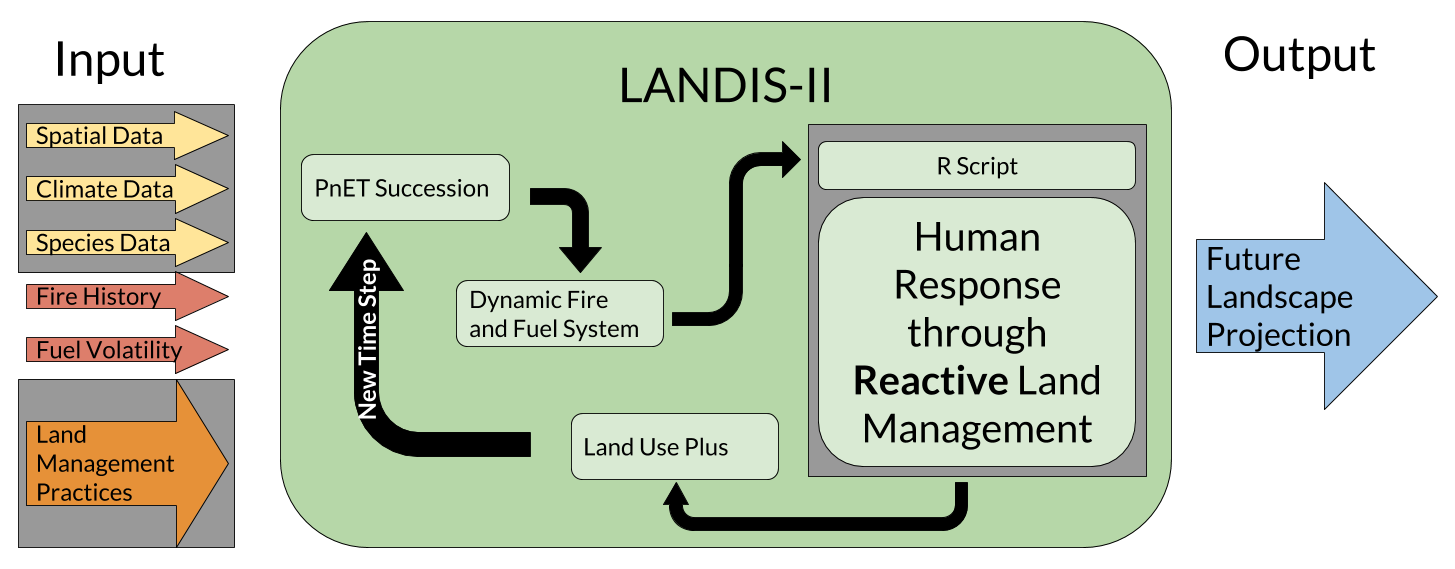
\includegraphics[width=\linewidth]{landis_what_i_did_final.png}
\end{frame}

\section{Climate Scenarios}
\subsection{}

\begin{frame}{Climate Scenarios}
%conditions under a recent trends scenario that samples historic trends yearly to produce the climate beyond 2010 and under the Intergovernmental Panel on Climate Change’s A2 scenario that describes a future with high populations, slow demographic transition, and substantial emissions due to delayed technological development (IPCC 2000)

% \begin{center}
		 \textbf{\color{climateChange}Climate Change }
			\begin{itemize}
				\item<a2@1-> describes a future with high populations, slow demographic transition, and substantial emissions due to delayed technological development
                \item<a2@1-> CO2 concentration is 390 parts per million in 2010 and \textbf{grows to 856 parts per million} in 2100
			\end{itemize}
            \vspace*{.75cm}
          \textbf{\color{recentTrends}Historic Climate} 
			\begin{itemize}
				\item<rt@1-> samples historic trends yearly to produce the climate beyond 2010
                \item<rt@1-> CO2 concentration set to a \textbf{constant 390 parts per million} beyond 2010 
			\end{itemize}
            
            
% \begin{columns}
%     \begin{column}{0.5\textwidth}

%     \end{column}
%     \begin{column}{0.5\textwidth}

%     \end{column}
% \end{columns}
% \end{center}
\vfill

\scriptsize{\textit{Data from Hostetler, S.W., J. R. Alder, \& A. M. Allan. 2011. Dynamically downscaled climate simulations over North America: Methods, evaluation, and supporting documentation for users: U.S. Geological Survey Open-File Report 2011-1238, 64 p\newline A2 Scenario from IPCC. 2010. Emission Scenarios. Cambridge University Press.}}
\end{frame}



\begin{frame}{Temperature}
\centering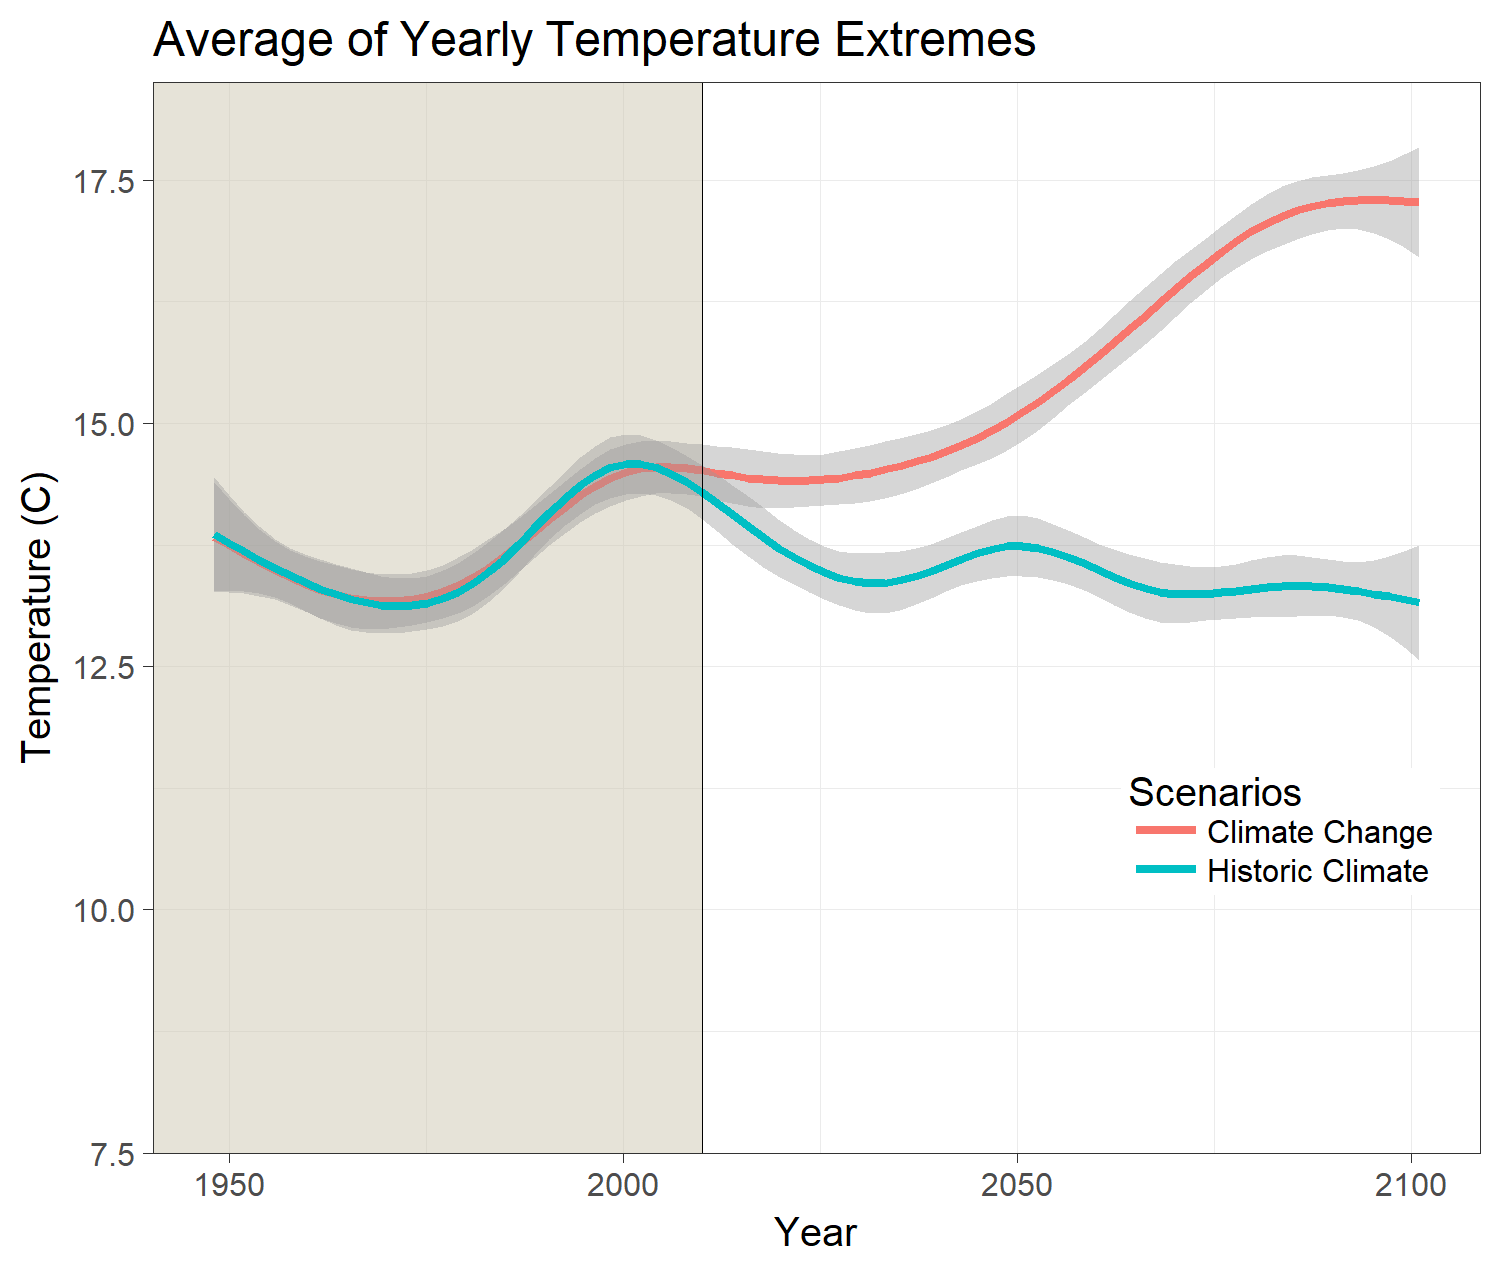
\includegraphics[width=.75\linewidth]{temp_fix_legend.png}
\end{frame}

\begin{frame}{Precipitation}
\centering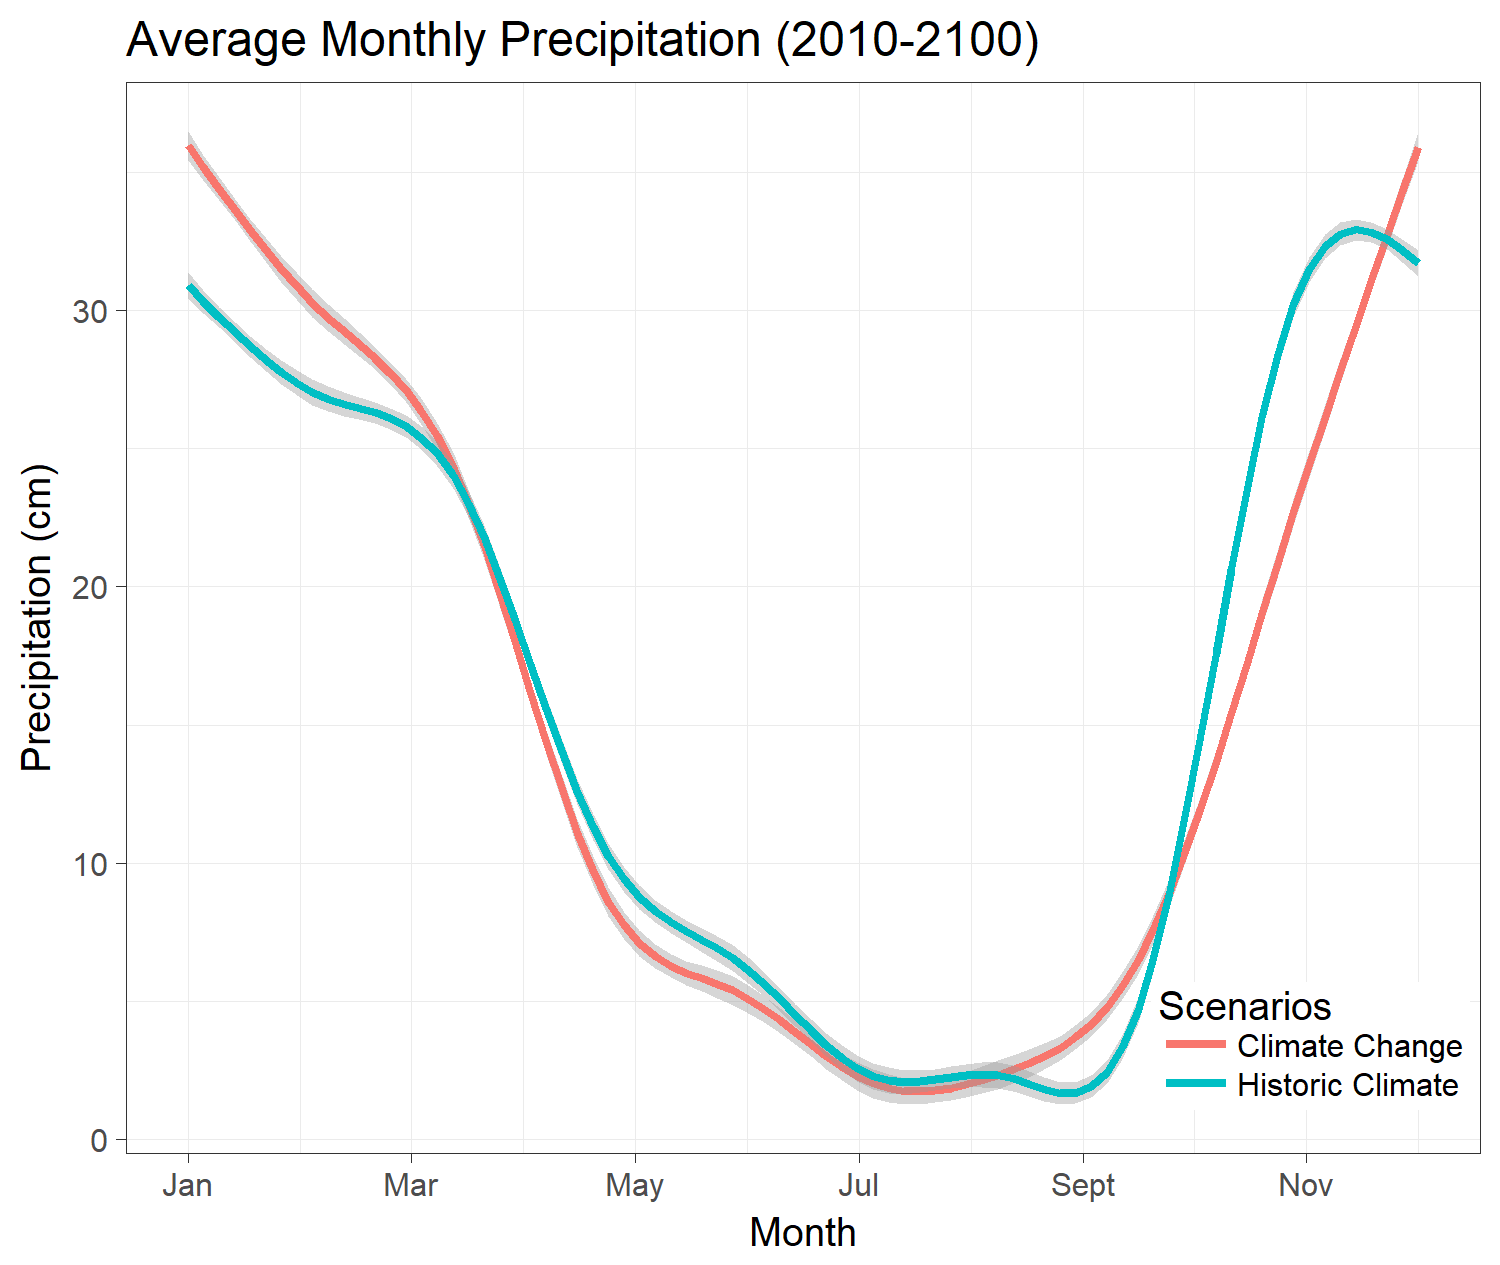
\includegraphics[width=.75\linewidth]{prec_legend_fix.png}
\end{frame}


\section{Simulating Human Response to Fire}
\subsection{}


\begin{frame}{Simulating Human Response: General Rules}
\begin{itemize}
\item   Cuts are effective for 15 years
\item   Land owned by the Forest Service maintains planned fuel breaks that follow low elevation areas
\item   \textbf{National Wilderness Areas are never cut}
\end{itemize}
\vspace*{.25cm}
\centering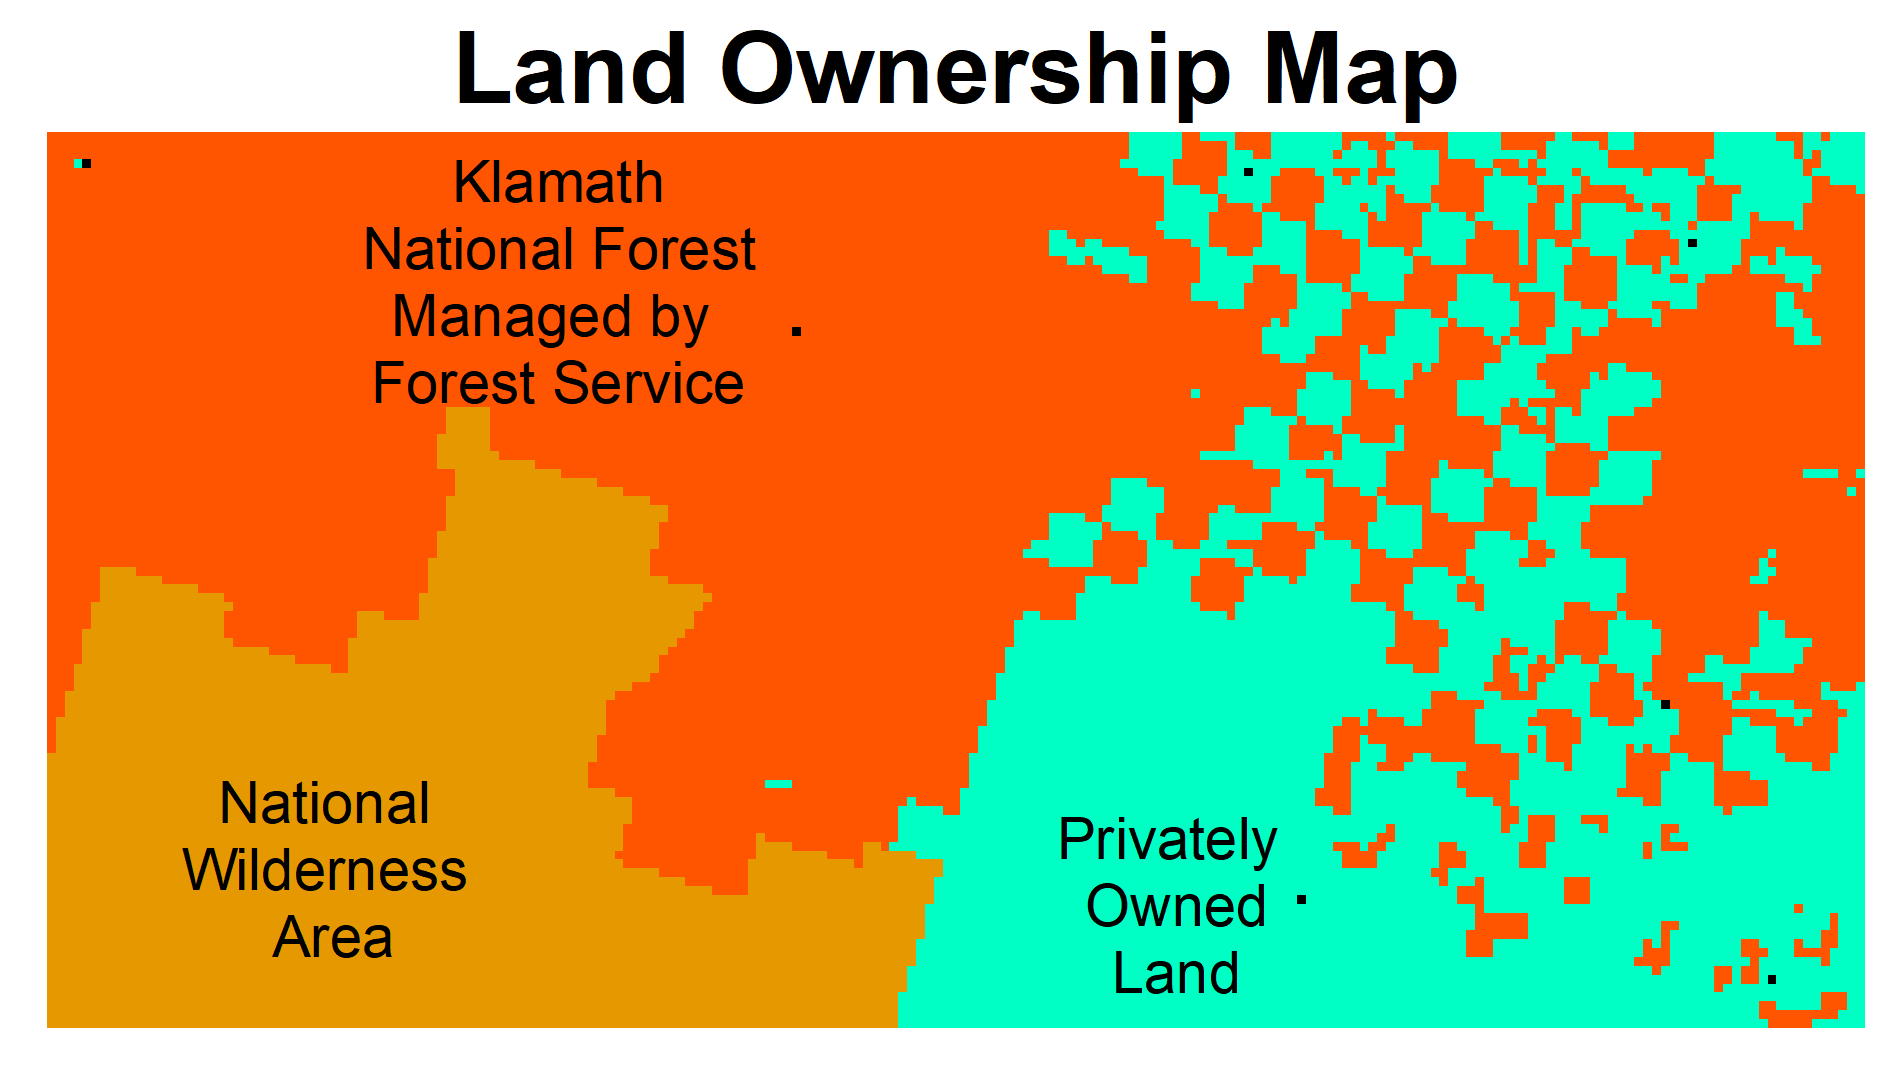
\includegraphics[width=.75\linewidth]{landOwnershipMap.png}
%More than 60 percent of the County is managed by Federal and State agencies

%The checkerboard pattern originated in the heyday of the railroads, when the federal government wanted to expedite the construction of a rail line from San Francisco to Portland. A checkerboard was drawn on the map, with the hoped-for railroad down the middle. In 1866, every alternating square of land was sold to homesteaders, while the remaining squares were ceded to the Oregon & California railroad with certain conditions: the timber was to be cut for the construction of the rail, and afterward, the cleared railroad land was also supposed to be sold to homesteaders for not more than $2.50 per acre. The railroads, however, did not sell most of the federally-donated lands as they were required, so Congress reclaimed 2,890,893 acres of the land in 1916 under the O&C Revestment Act. Eventually, the Bureau of Land Management was created to manage federally owned lands for cattle and sheep grazing, timbering, mining, and so forth.

%Railroad land grants split the land surrounding the area where train tracks were to be laid into a checkerboard pattern. The land was already divided into 640-acre numbered sections according to the Public Land Survey System; odd-numbered plots were given to private railroad companies and the federal government kept even-numbered plots.

\end{frame}

\begin{frame}{Simulating Human Response: Basic Idea}
\begin{itemize}
\item[] \textbf{\color{fuelBreakColor}Proactive Response }
\begin{itemize}
\item	\textbf{Fuel breaks} implemented to divide large groups of connected fuel types 
\end{itemize}
\vspace*{.25cm}
\item[] \textbf{\color{salvageLogColor}Reactive Response}
\begin{itemize}
\item	Post fire \textbf{salvage logging} was performed on burnt cells and their neighbors if the cells were hit by a fire of severity level between 1 and 3 (where a level 5 fire kills all trees in the cell)
\end{itemize}
\vspace*{.25cm}
\item[] \textbf{\color{fuelReductionColor}Mixed Response }
\begin{itemize}
\item	Land around developed areas was \textbf{thinned} if there were fires present in more than half the cells in a 9-cell (2.43 km) diameter circle of the developed area
\end{itemize}
\end{itemize}
\end{frame}


\begin{frame}{Some Examples}
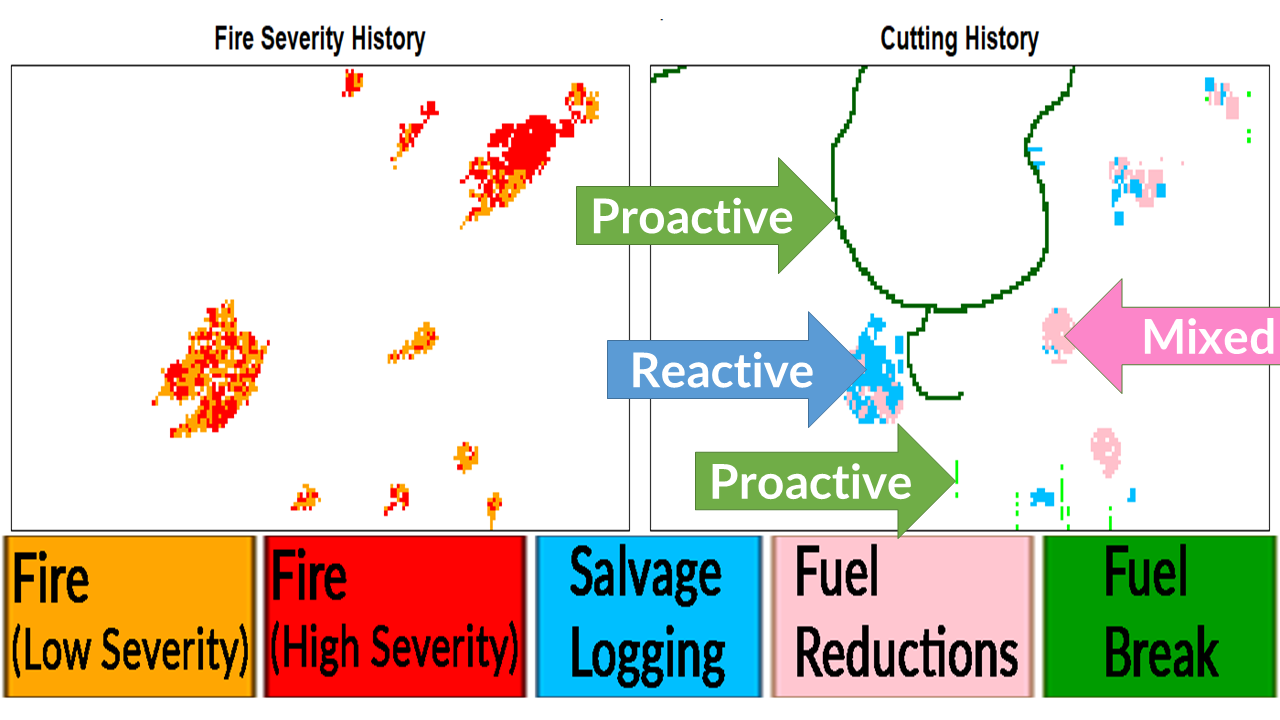
\includegraphics[width=\linewidth]{ExampleCut.png}
\end{frame}

\begin{frame}{Reactive Actions: Cutting in Response to Fire}
\centering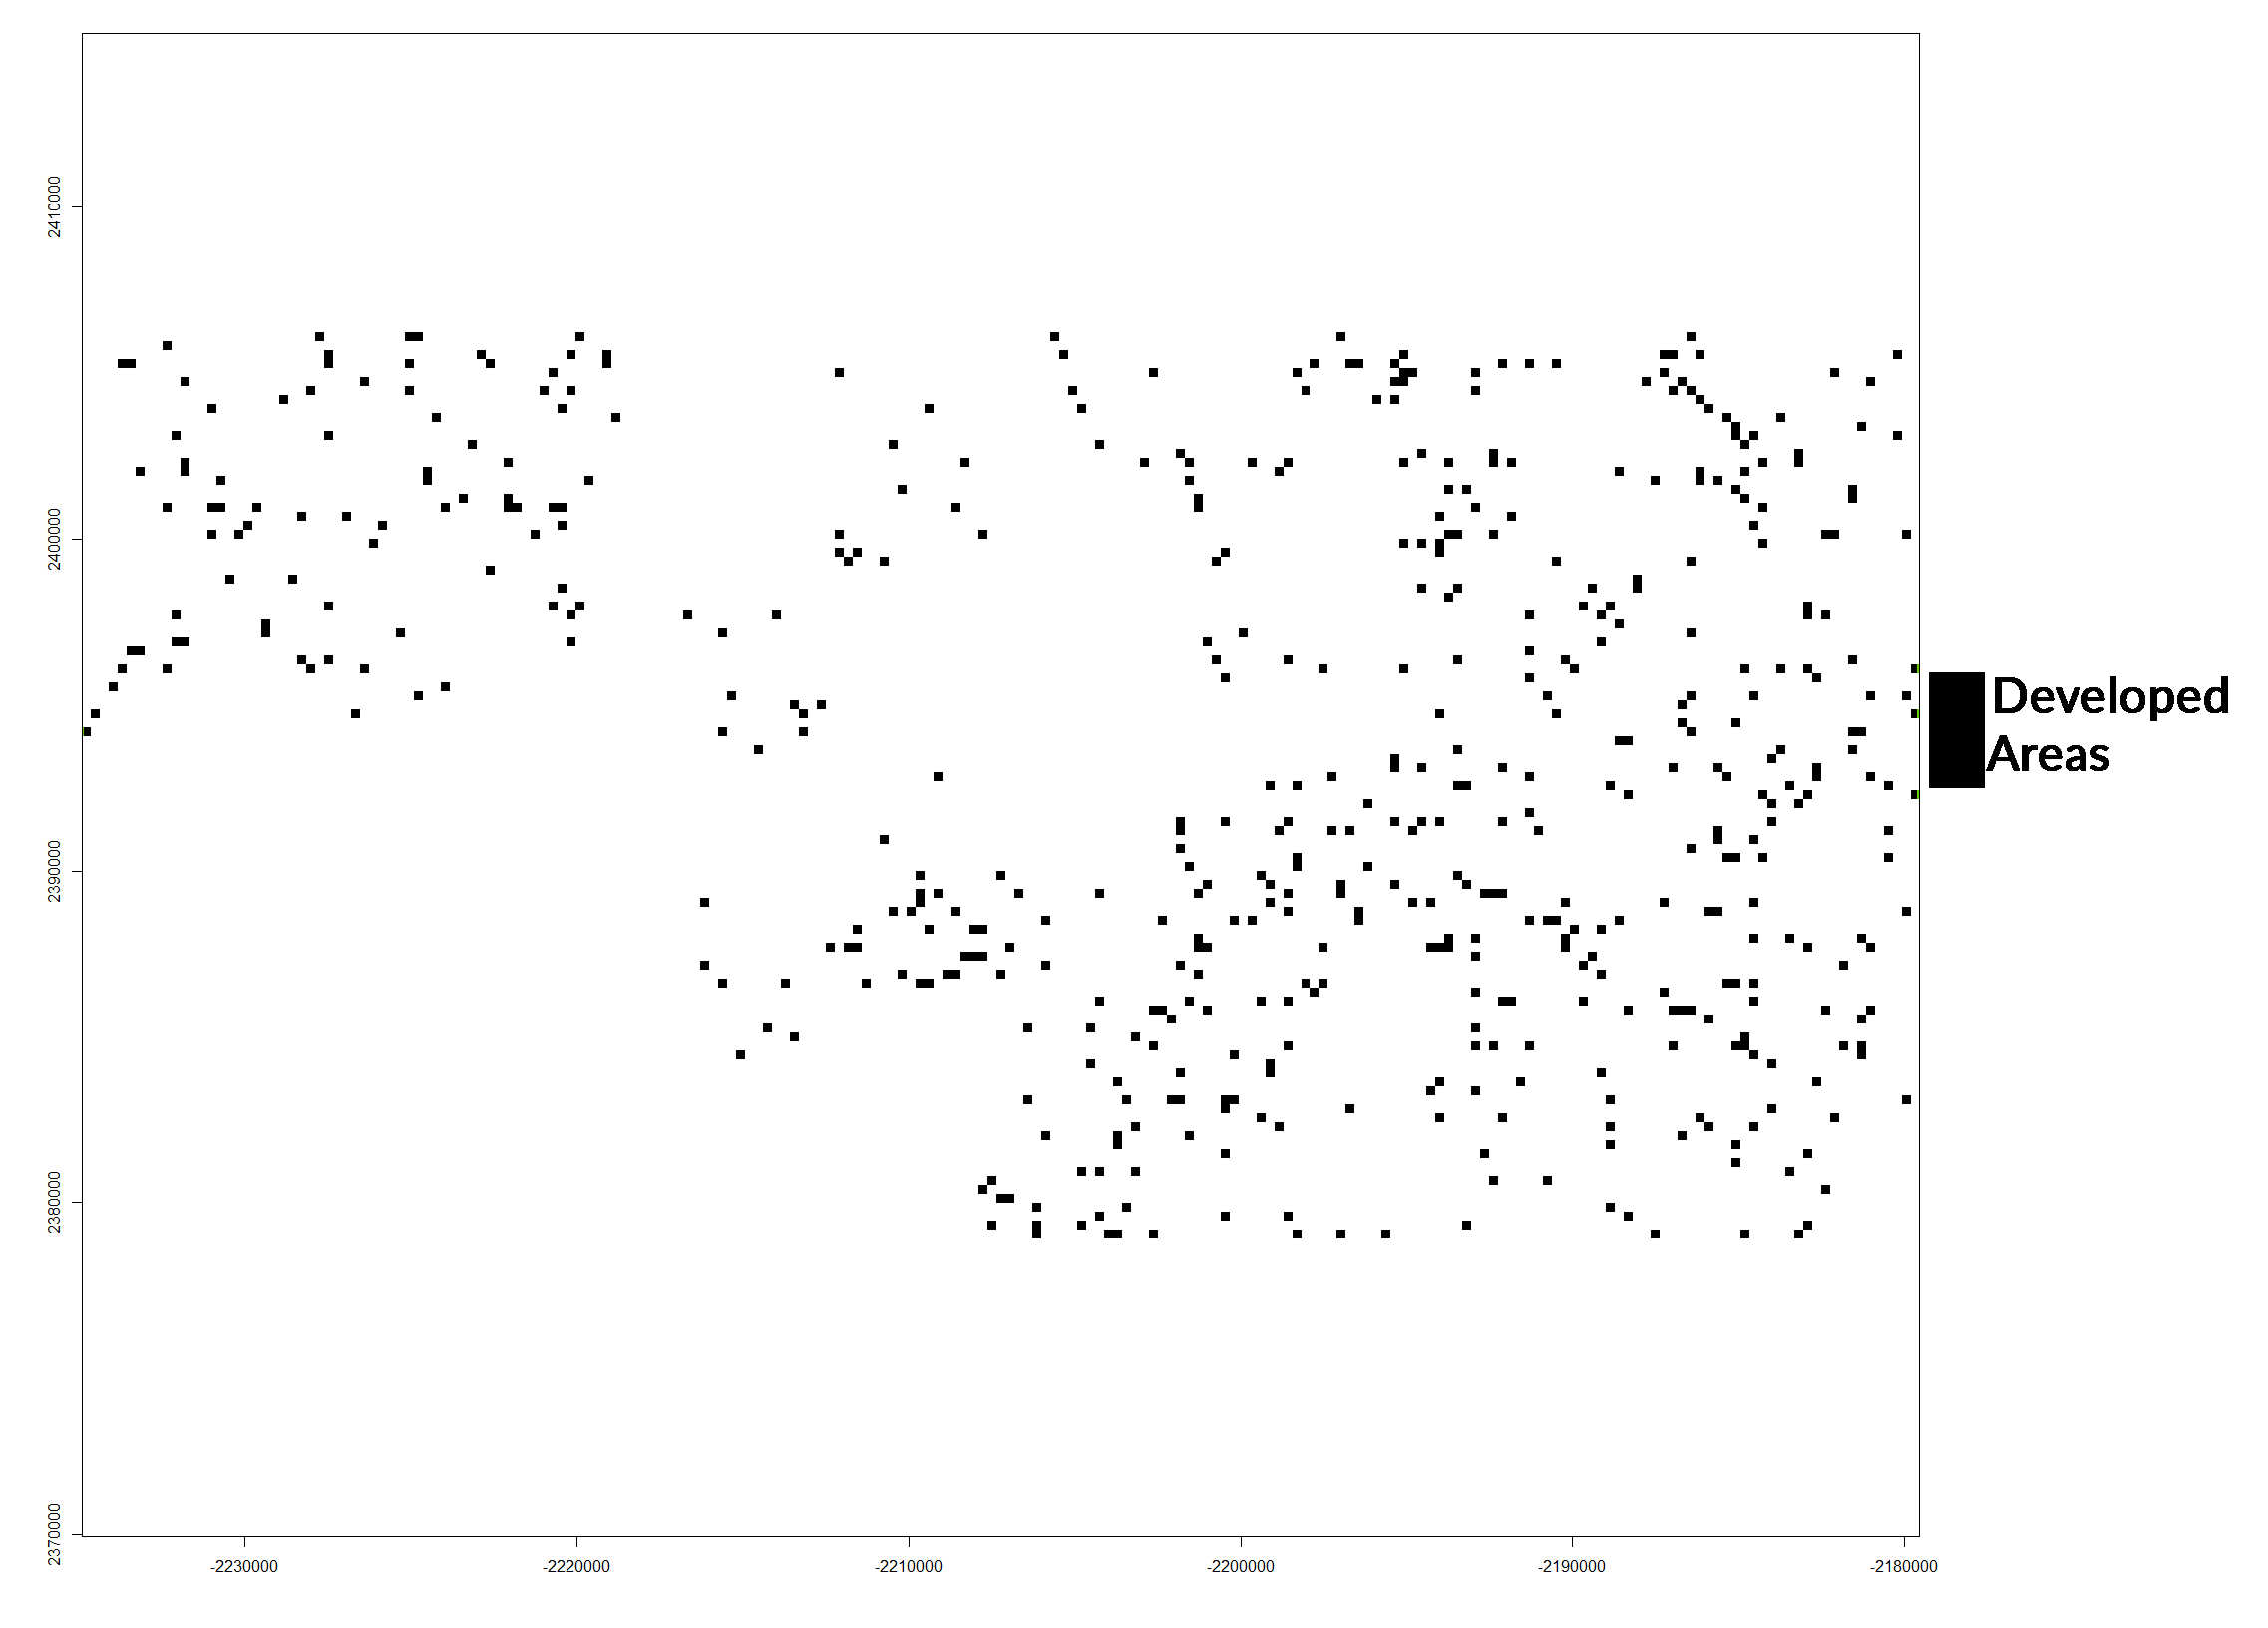
\includegraphics[width=.85\linewidth]{developAreaMap.png}
\newline
\scriptsize{\textit{Data from USGS Land Cover Data Viewer}}
\end{frame}

\begin{frame}{Reactive Actions: Cutting in Response to Fire}
\centering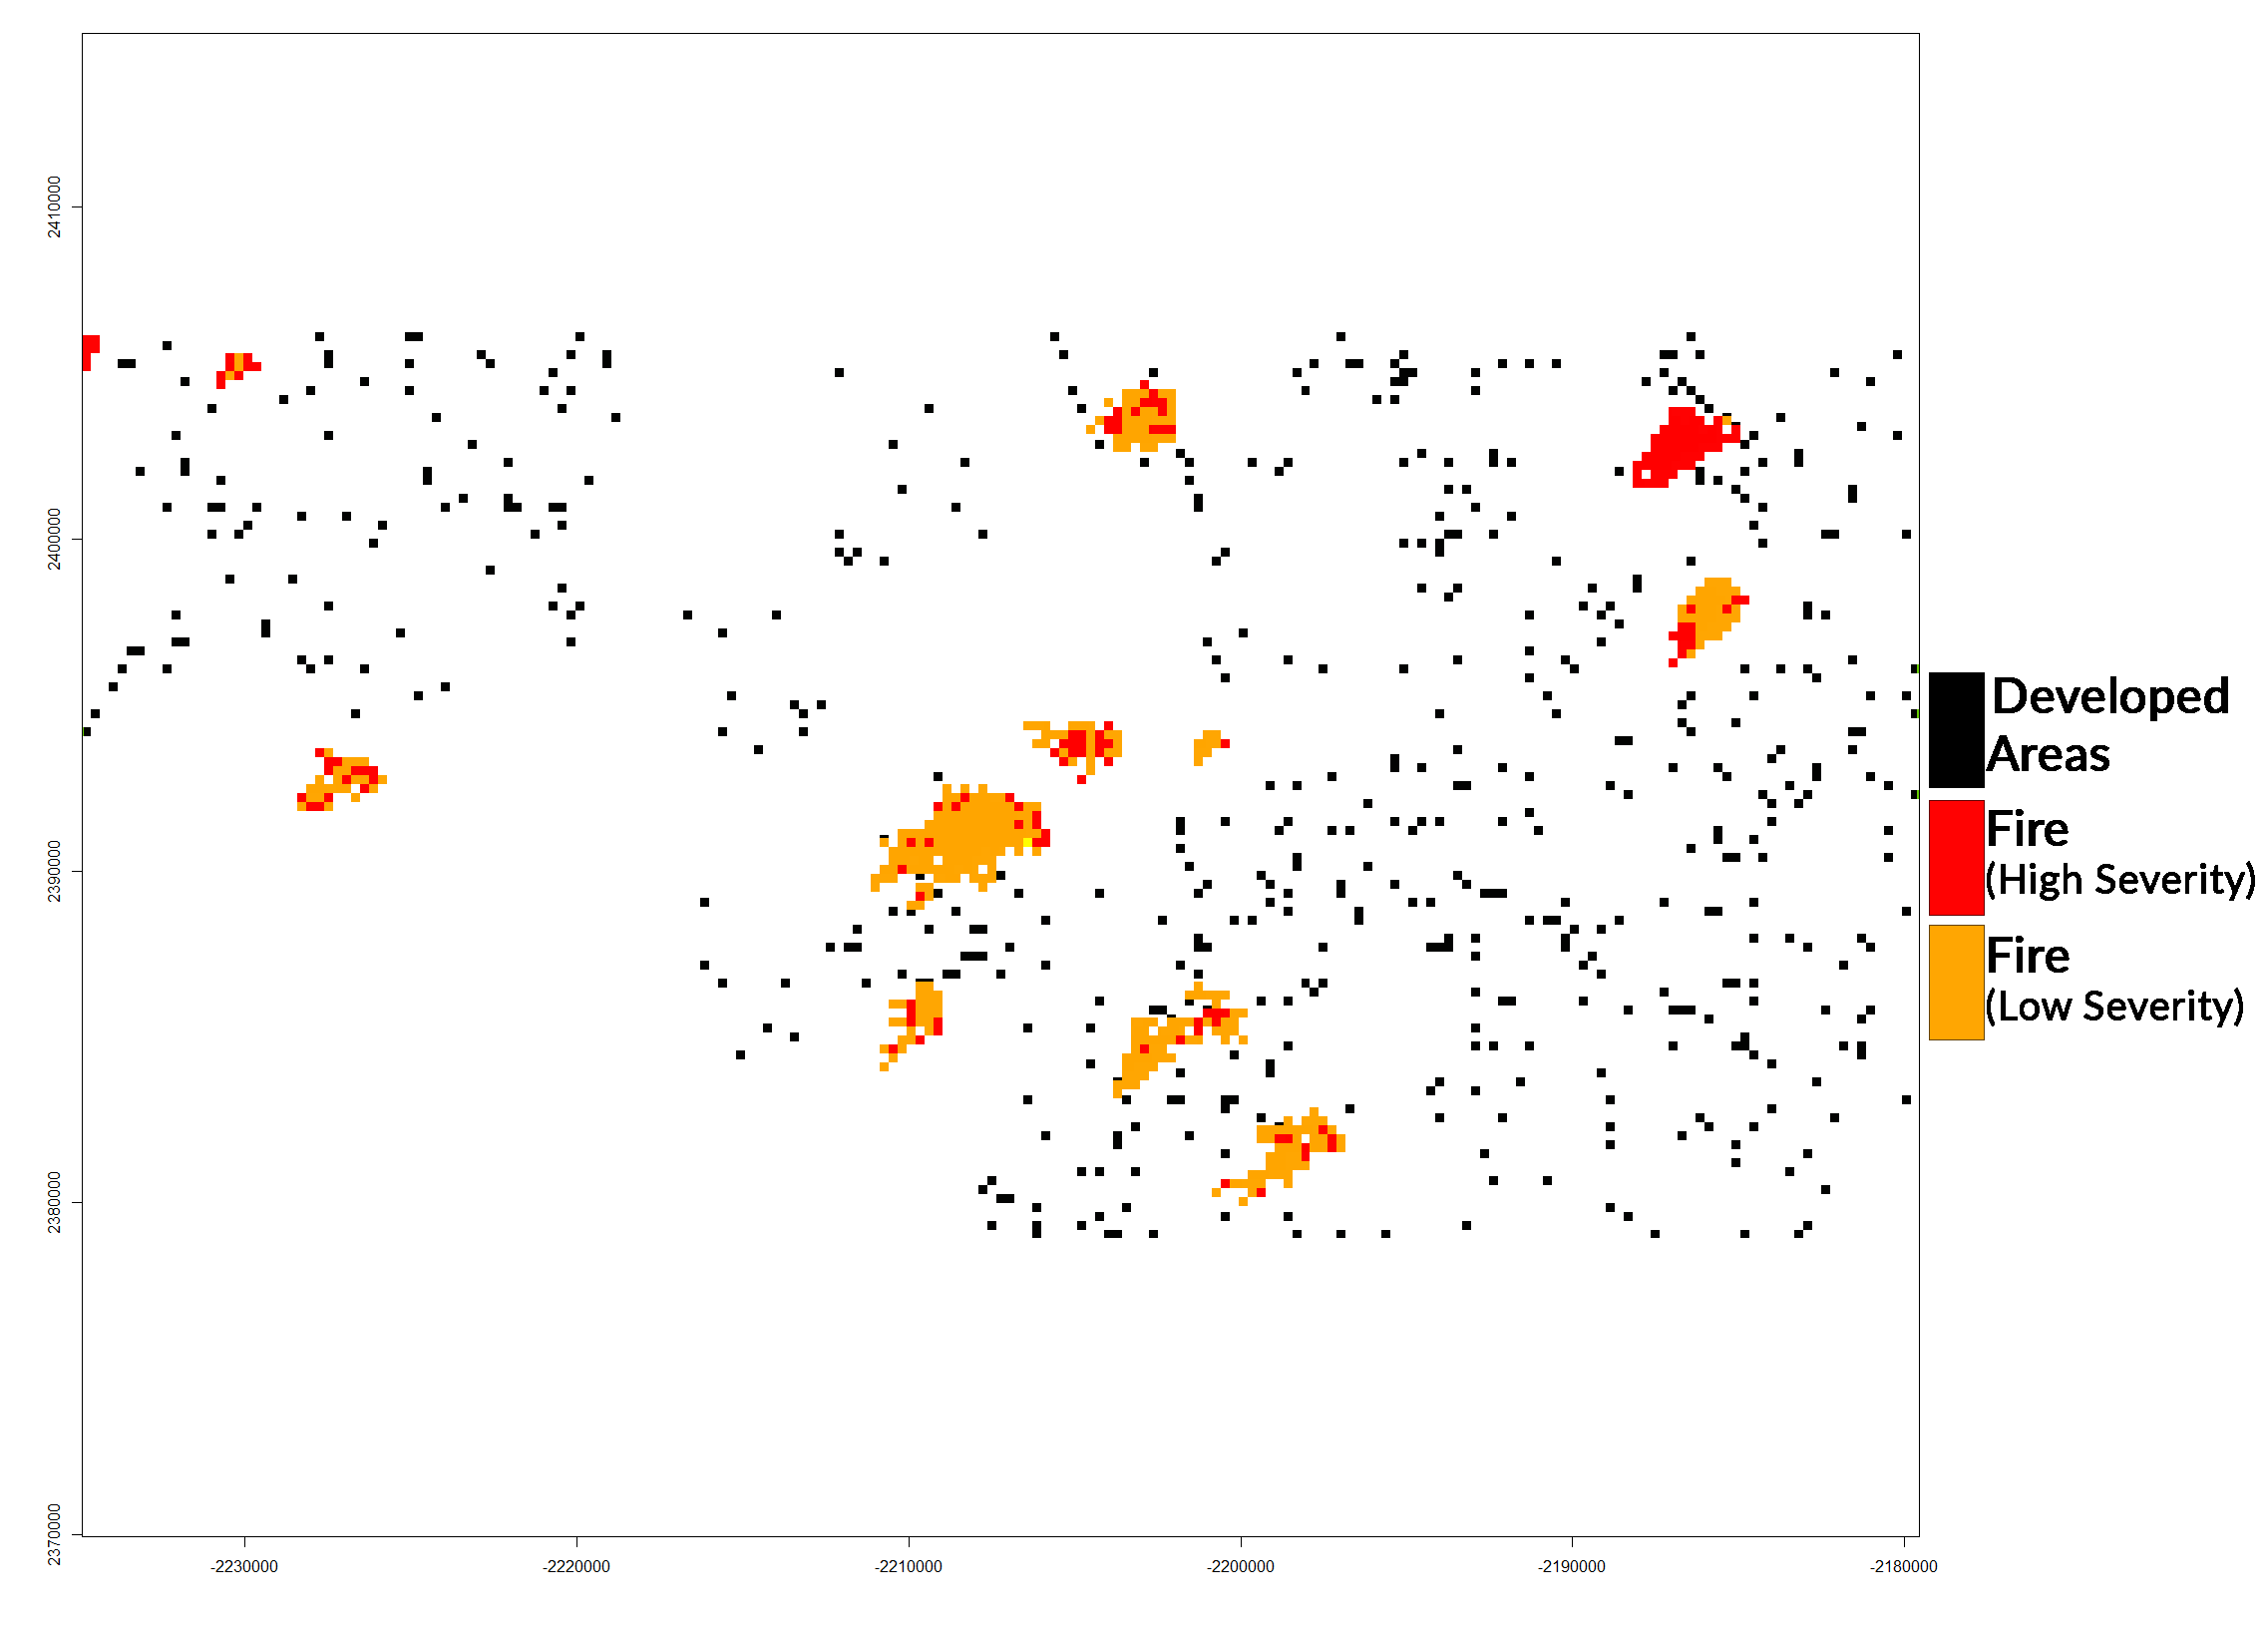
\includegraphics[width=.9\linewidth]{developAreaMapwithFire.png}
\end{frame}

\begin{frame}{Reactive Actions: Cutting in Response to Fire}
\centering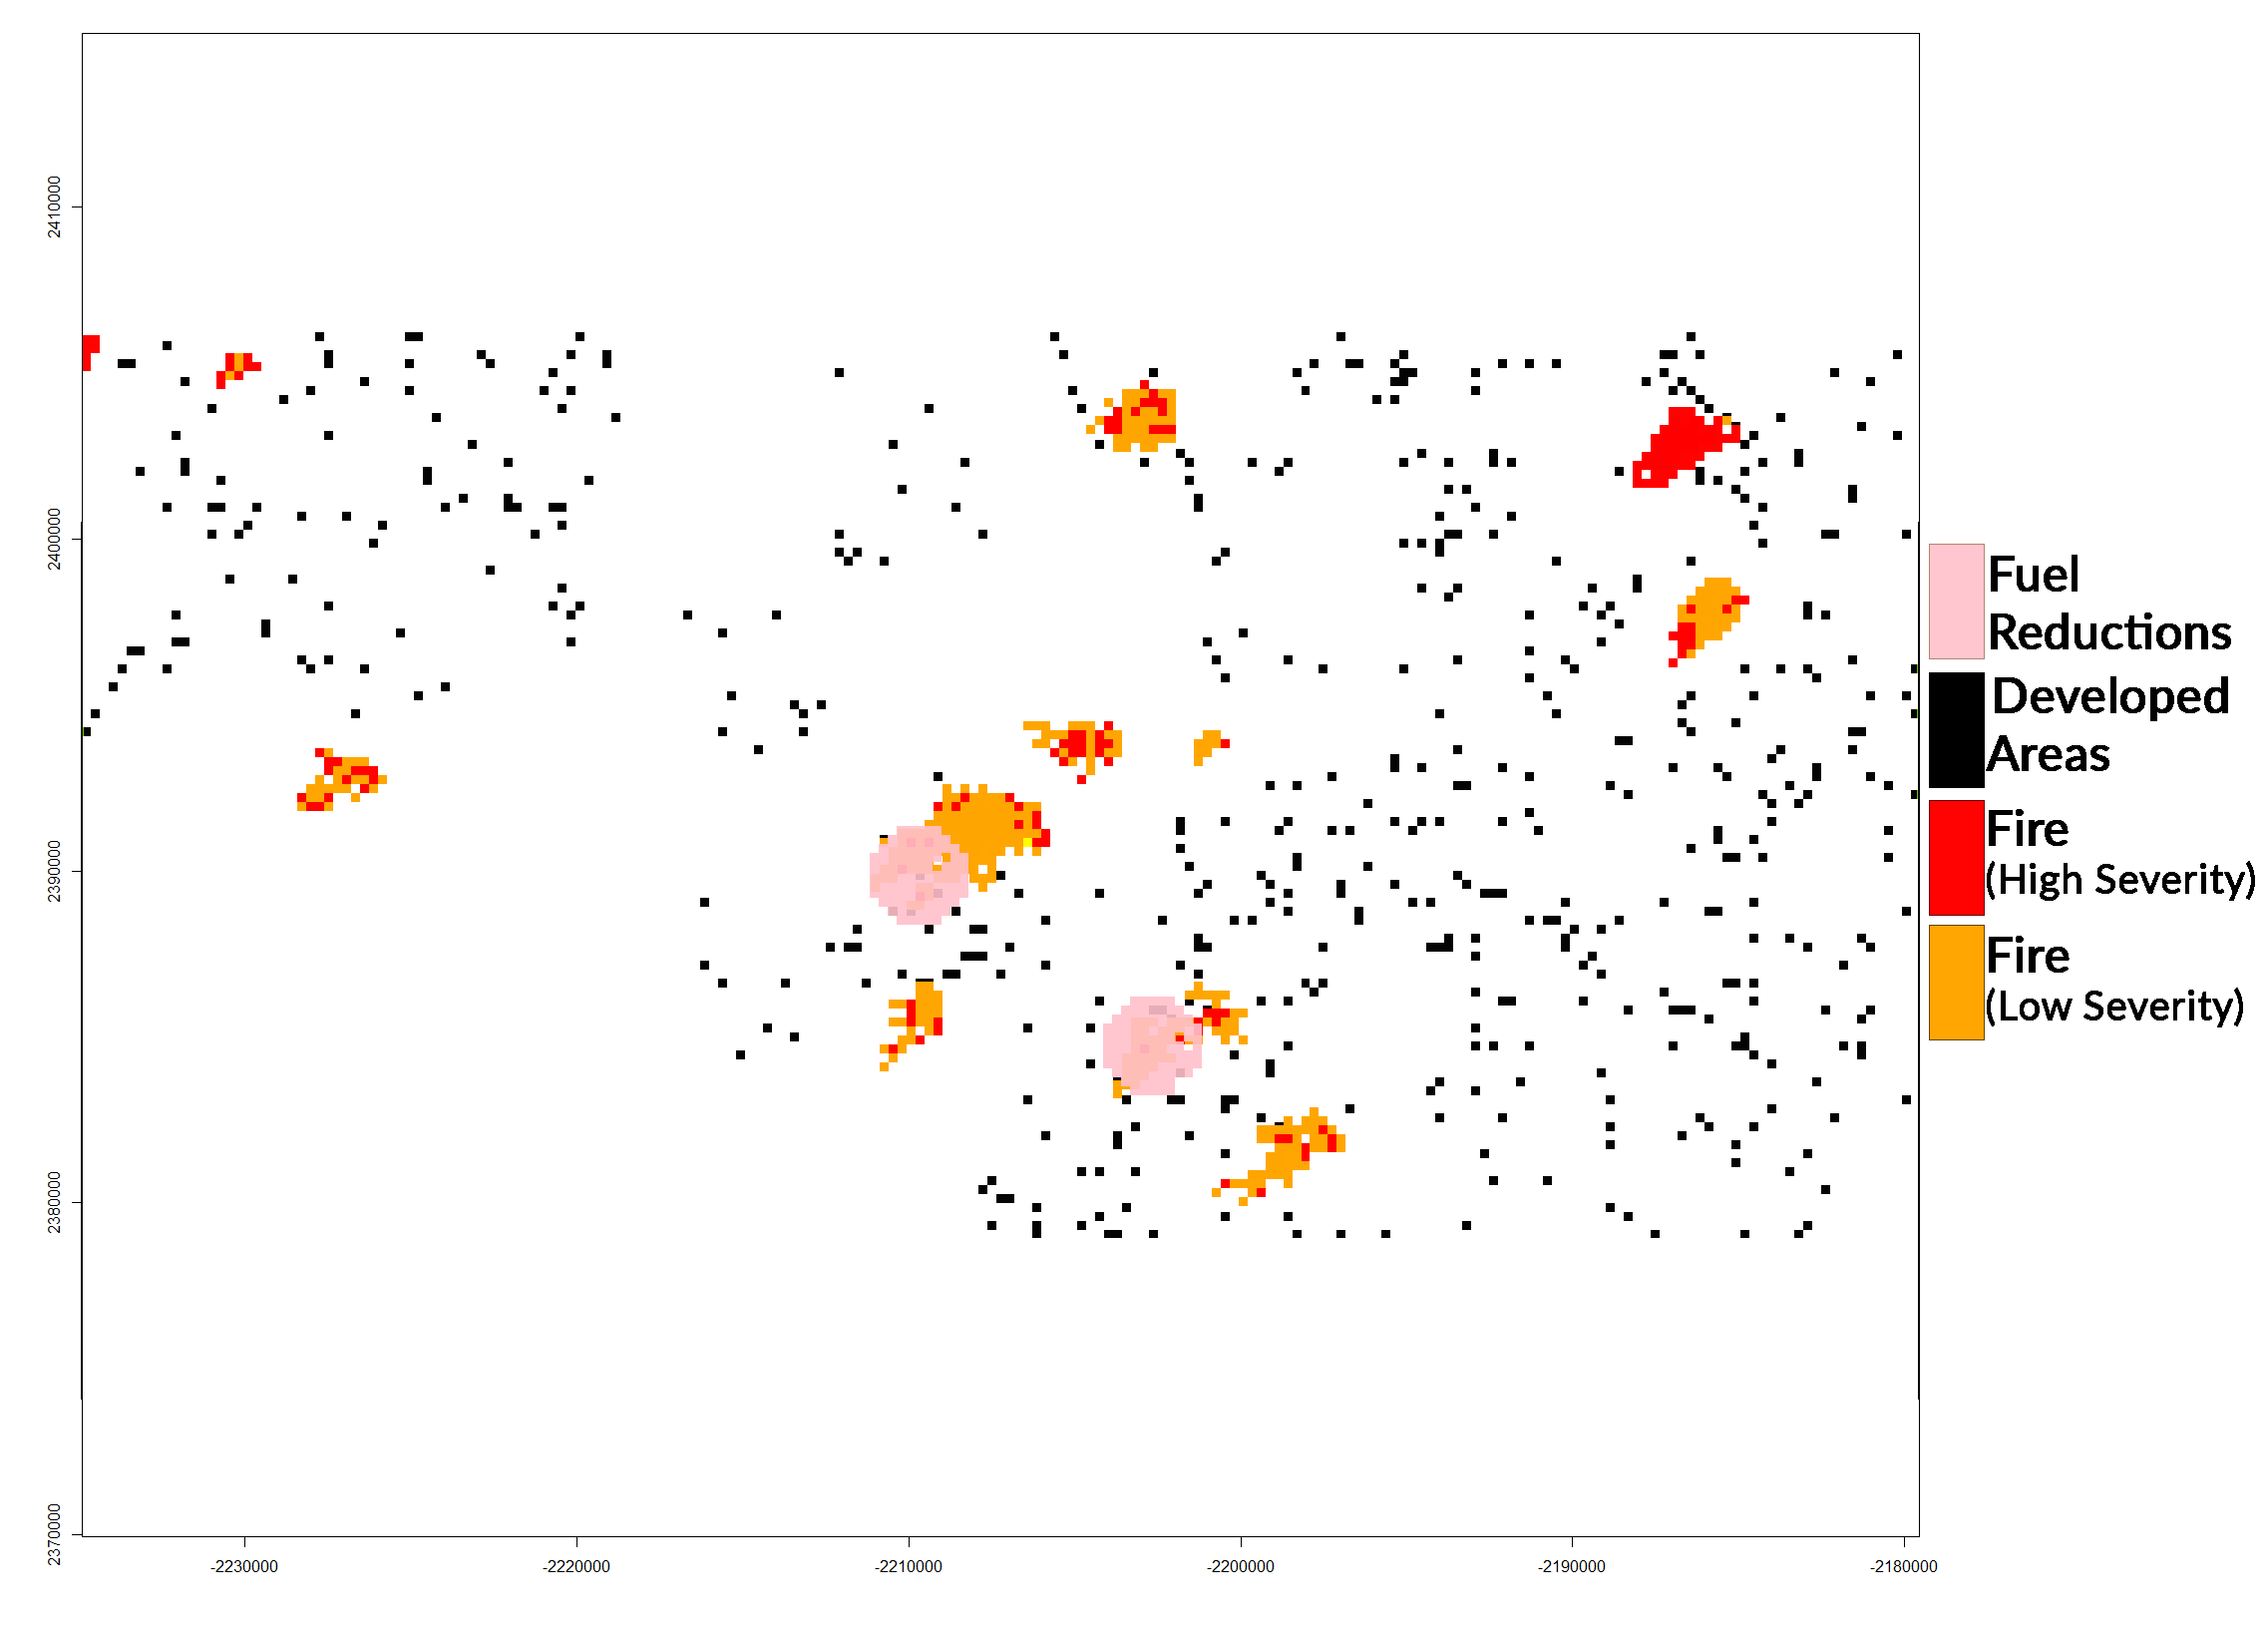
\includegraphics[width=.9\linewidth]{developAreaMapwithFireAndThinning.png}
\end{frame}

\begin{frame}{Reactive Actions: Cutting in Response to Fire}
\centering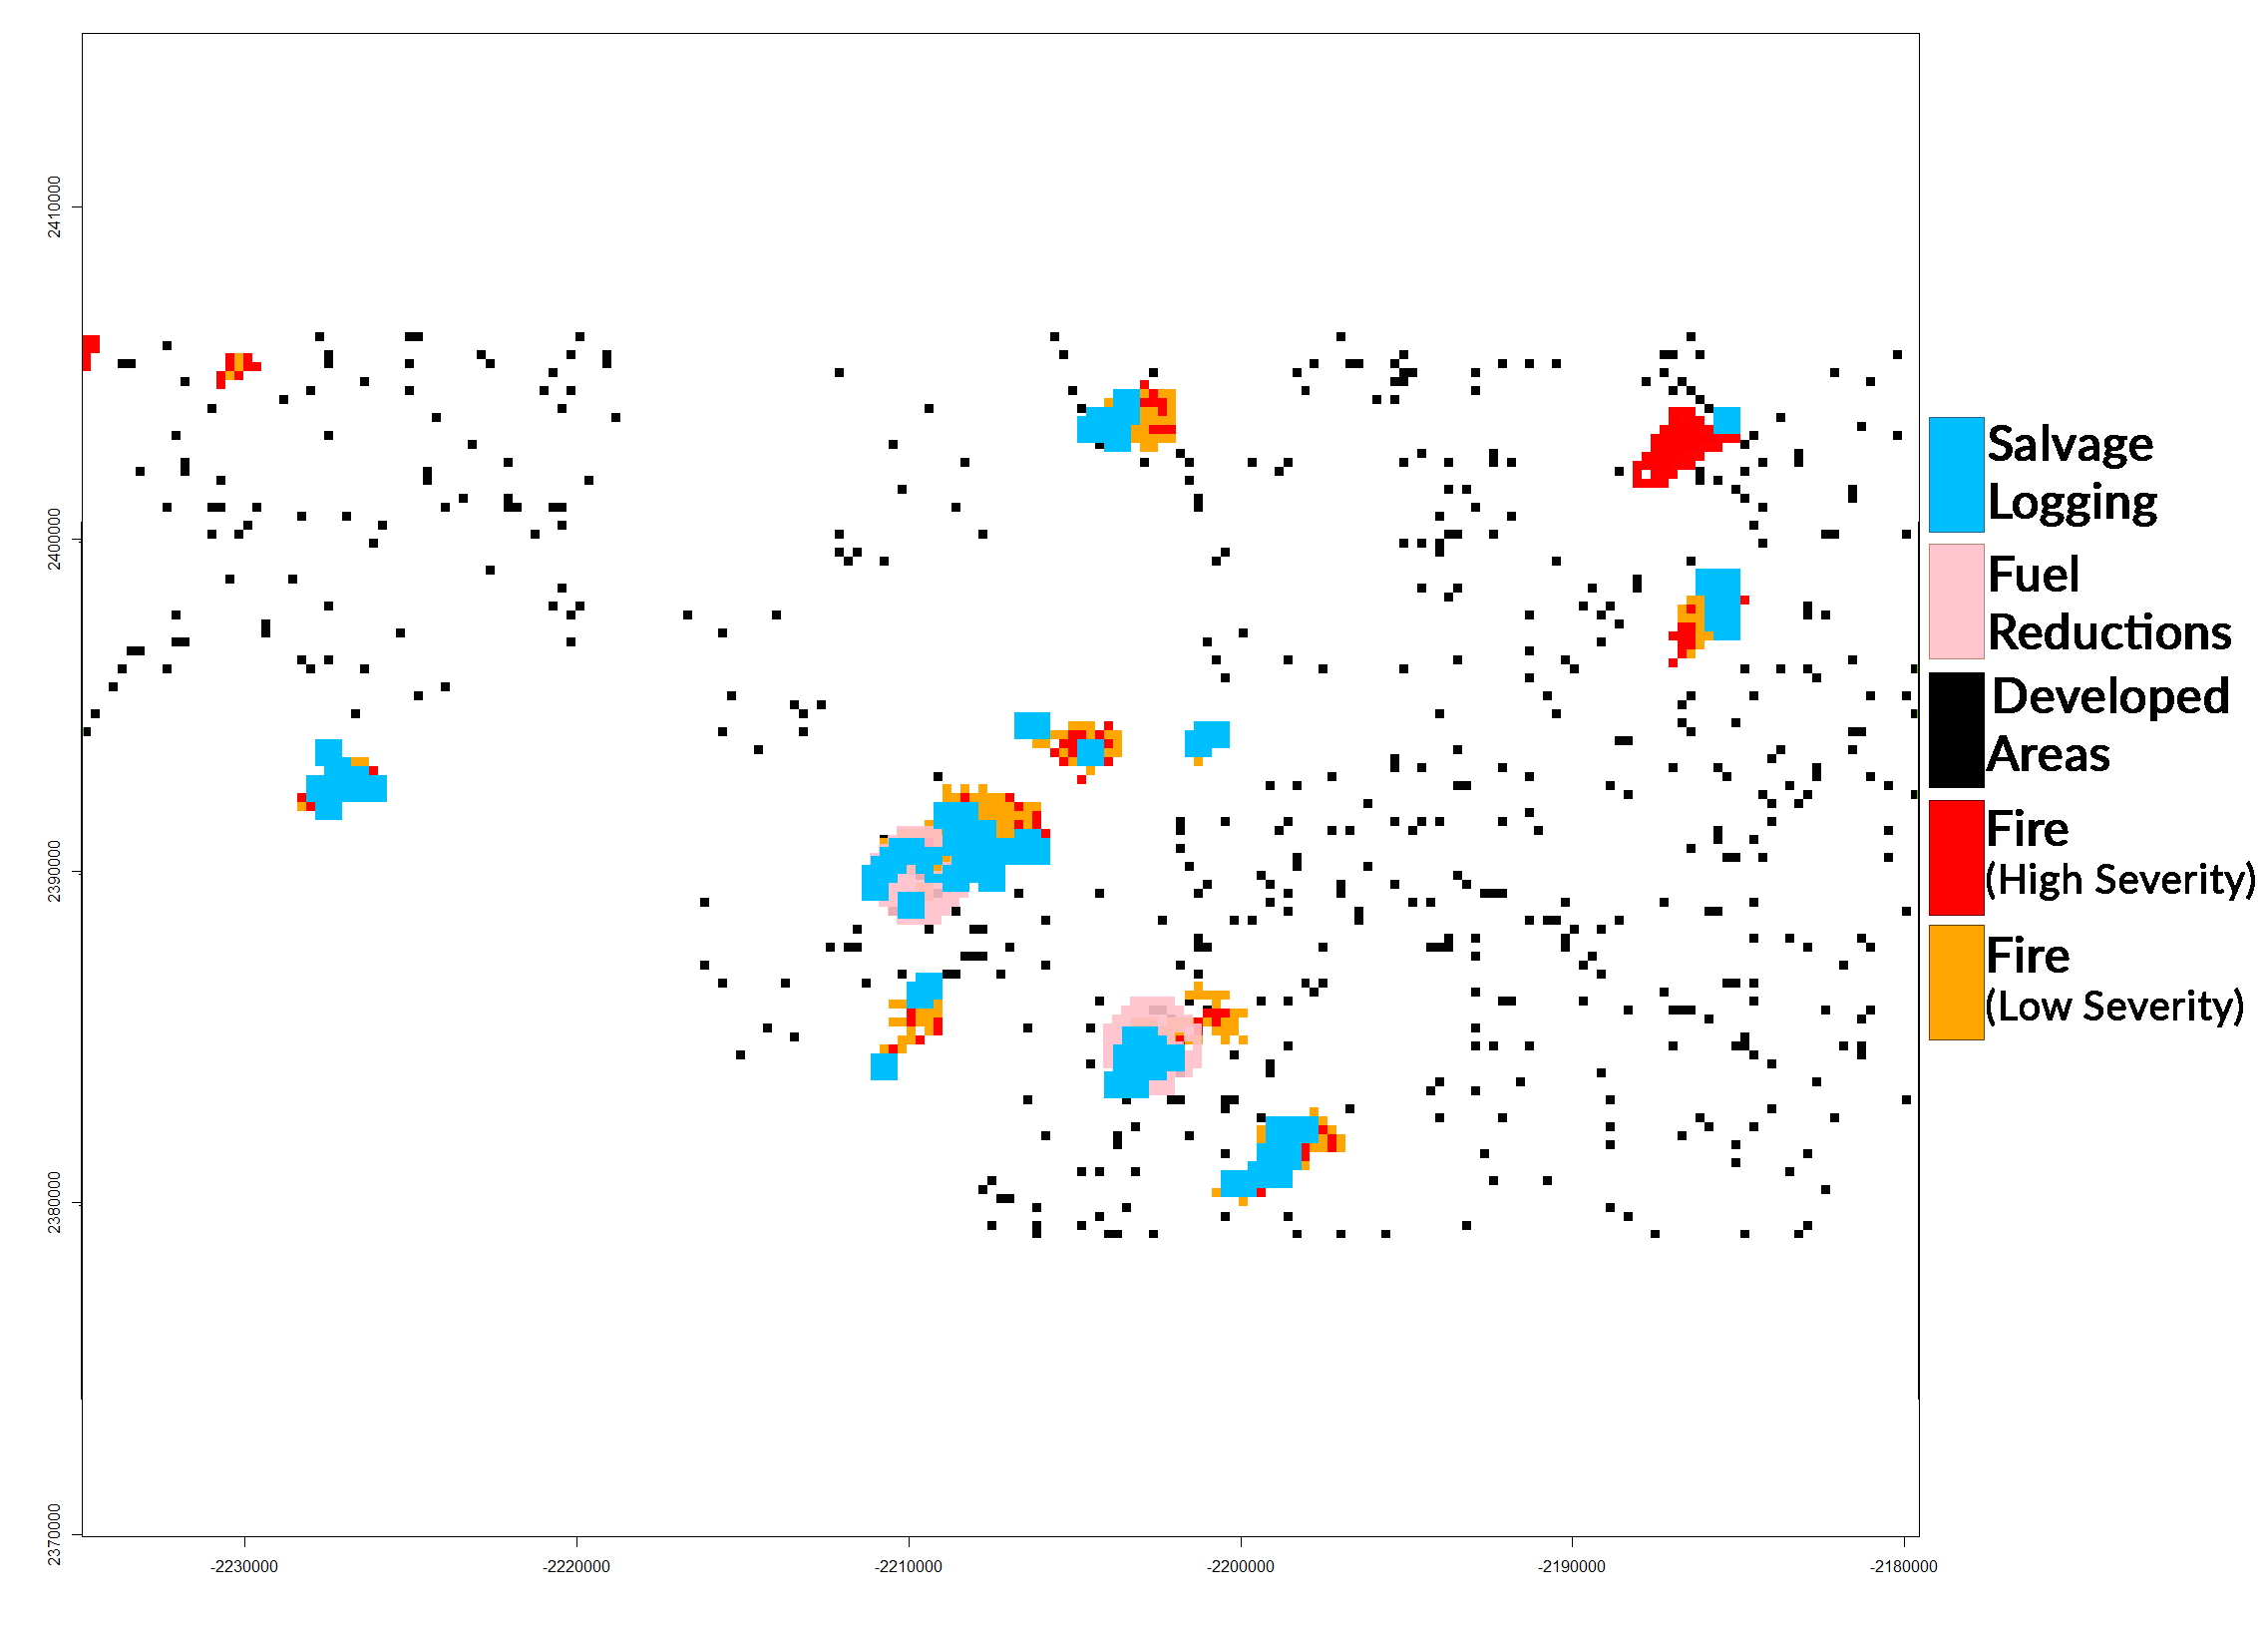
\includegraphics[width=.9\linewidth]{developAreaMapwithFireAndThinningAndSalvage.png}
\end{frame}

\begin{frame}{Proactive Actions: Reducing Connected Fuels}
\centering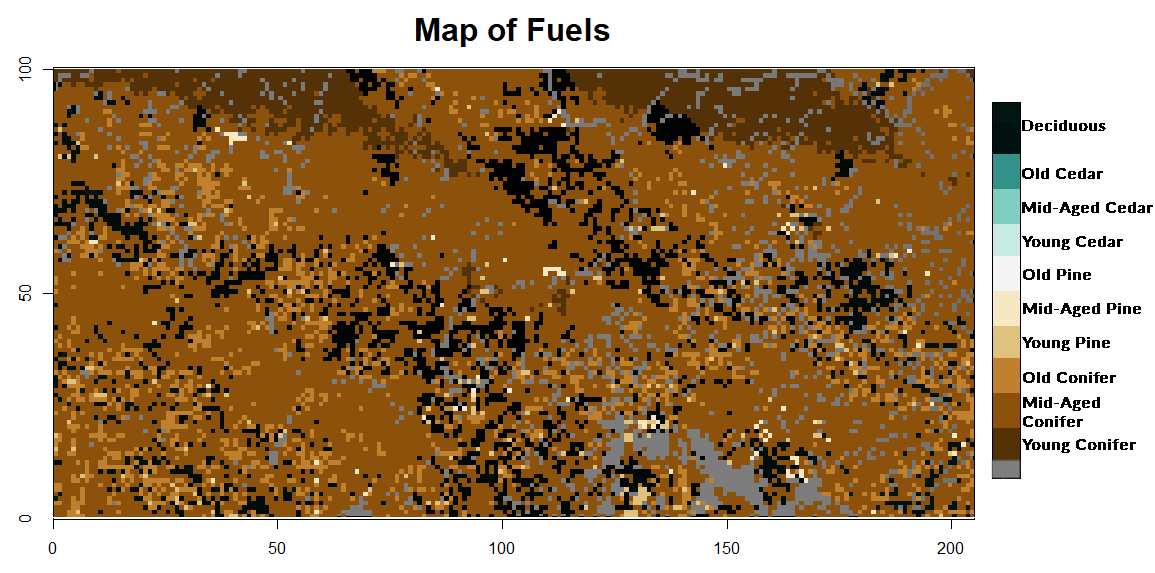
\includegraphics[width=\linewidth]{mapOfFuelFinallabel.png}
\end{frame}

\begin{frame}{}
\centering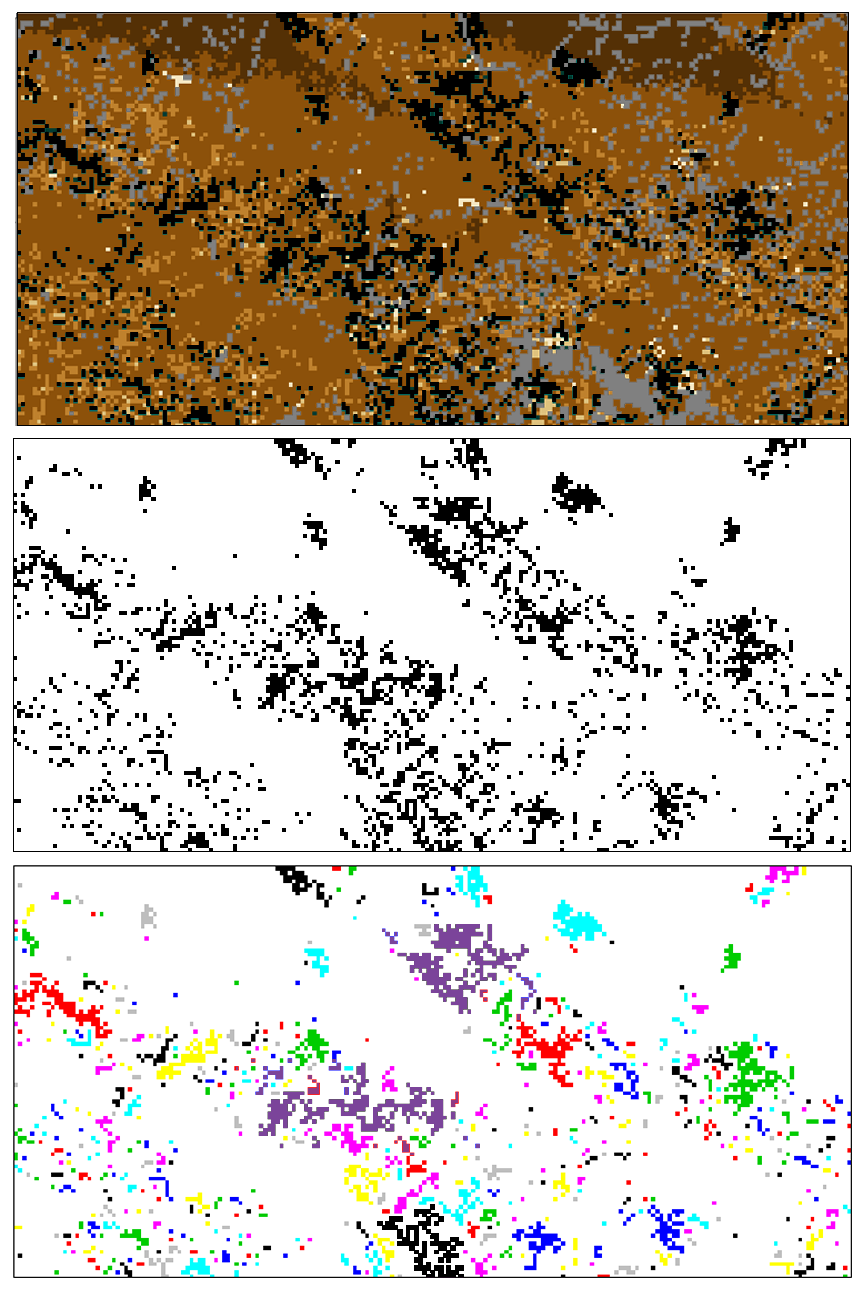
\includegraphics[width=.49\linewidth]{fuelMapTOConnectCompsFOREXAMPLE.png}
\end{frame}

\begin{frame}{Breaking up Connected Fuels}
\centering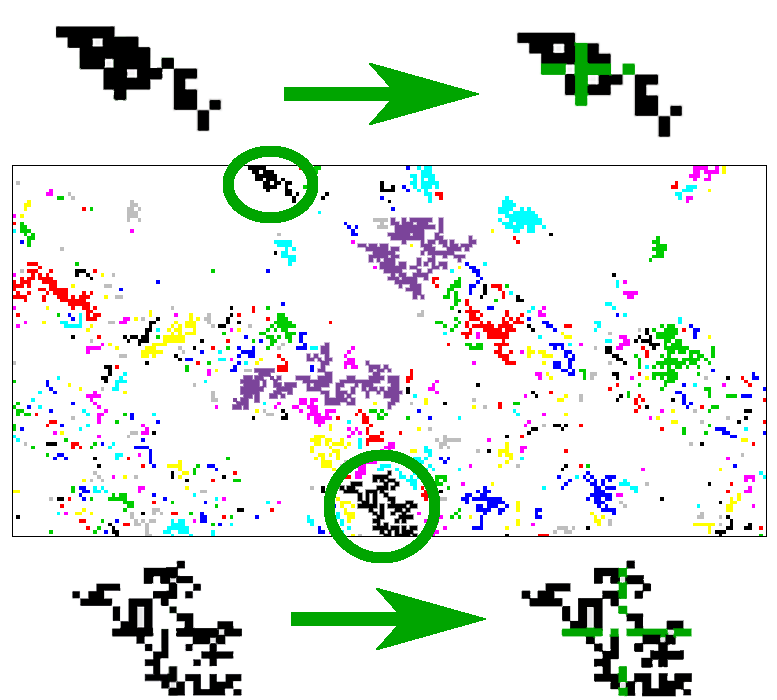
\includegraphics[width=.7\linewidth]{making_connected_graph_picutre.png}
\end{frame}

\begin{comment}


\section{Putting all the Pieces Together}
\subsection{}
\begin{frame}{Aboveground Biomass}
\centering\includegraphics[width=.75\linewidth]{totalAGBFinal2.png}

%   Time    Total                                                  sim
%10   90 24979.74 sa3_FilledICs_REPS_10YTS__BASE__NOClimate/replicate1
%20   90 21022.96     sa3_FilledICs_REPS_10YTS__JUSTFIRE_NO/replicate1
%30   90 19833.06      sa3_FilledICs_REPS_10YTS__LU_FIRE_NO/replicate1
%40   90 38057.25   sa3_FilledICs_REPS_10YTS_BASE_A2Climate/replicate1
%50   90 33057.33      sa3_FilledICs_REPS_10YTS_JUSTFIRE_A2/replicate1
%60   90 29874.79       sa3_FilledICs_REPS_10YTS_LU_FIRE_A2/replicate1
\end{frame}


\begin{frame}{Affected Area}
\centering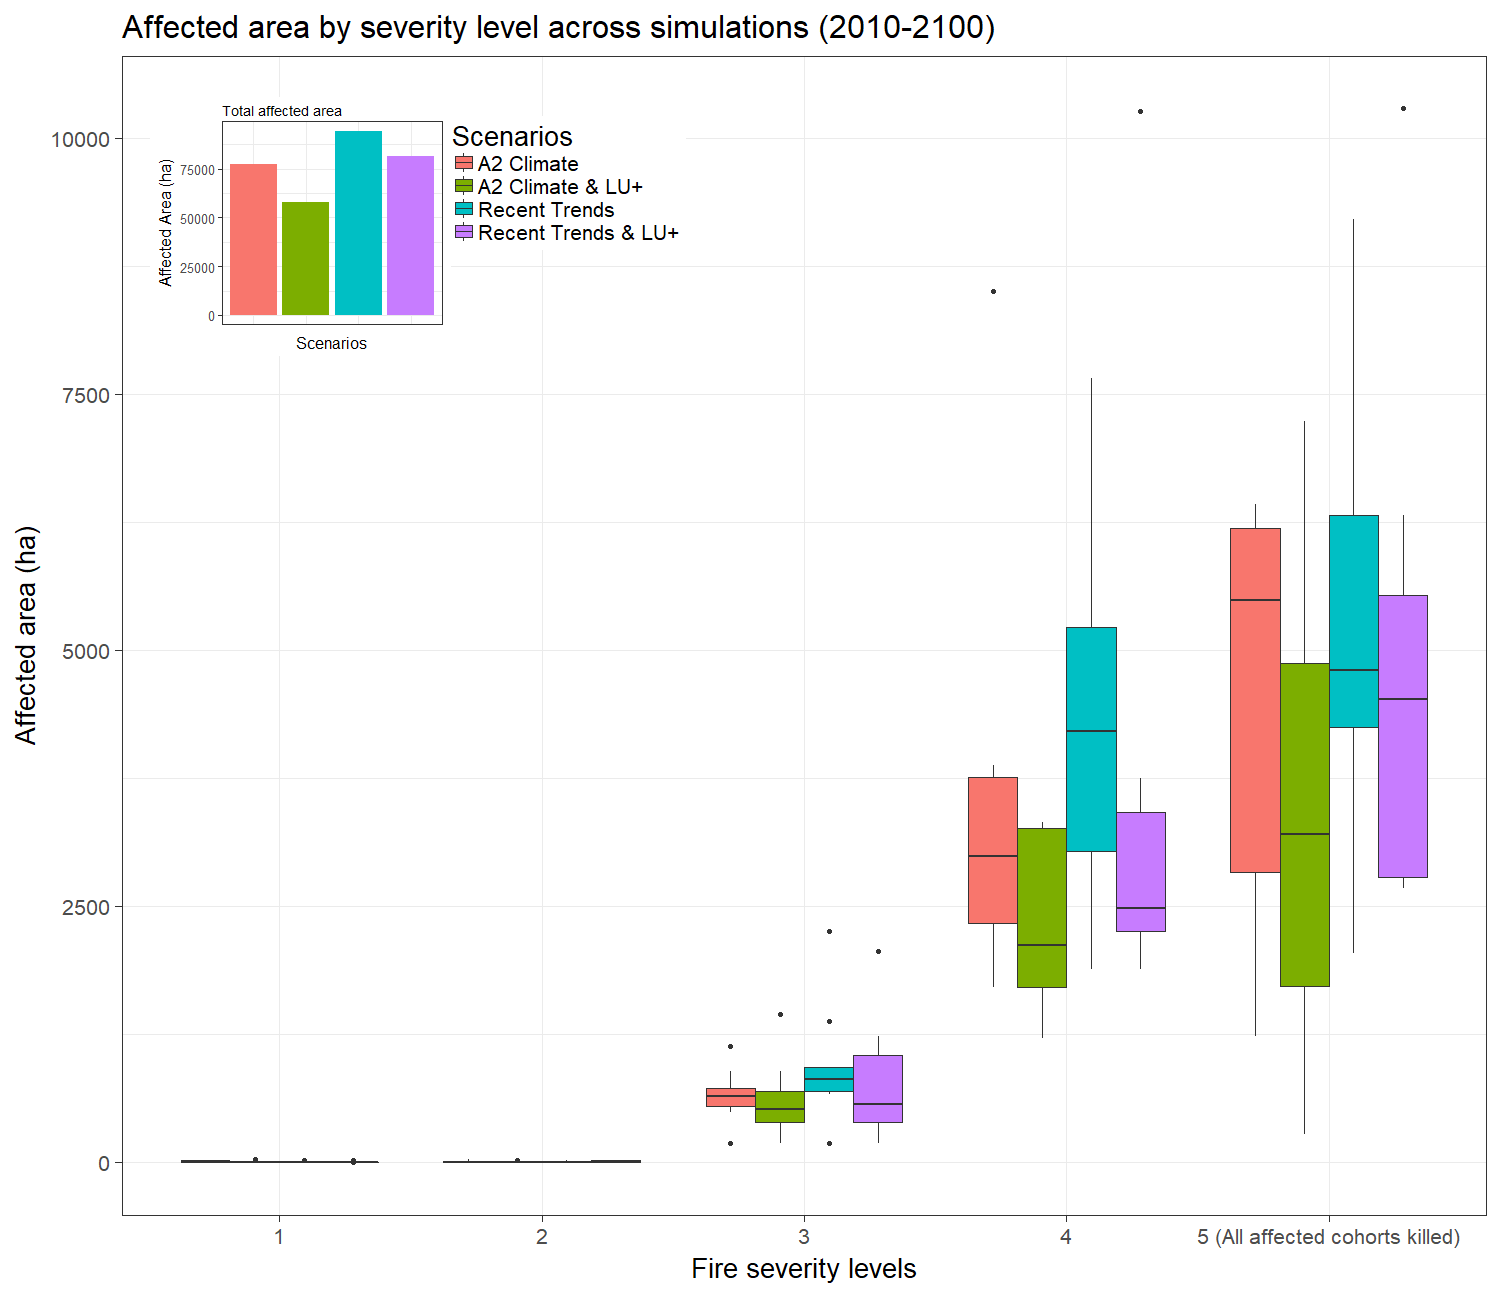
\includegraphics[width=.75\linewidth]{Affected_area_by_severity_level_across_simulations__2010-2100_.png}
\end{frame}



\begin{frame}{Effects of Human Response}
\centering\includegraphics[width=\linewidth]{firePerCellFinal.png}
\end{frame}
\end{comment}

\begin{comment}


\begin{frame}{Fire and Cut History}
\vspace*{-.05in}
\begin{figure}
\centering
\begin{subfigure}{.6\linewidth}
  \centering
 \includegraphics[width=.85\linewidth]{Human_response_History.png}
\end{subfigure}%
\begin{subfigure}{.4\linewidth}
  \centering
 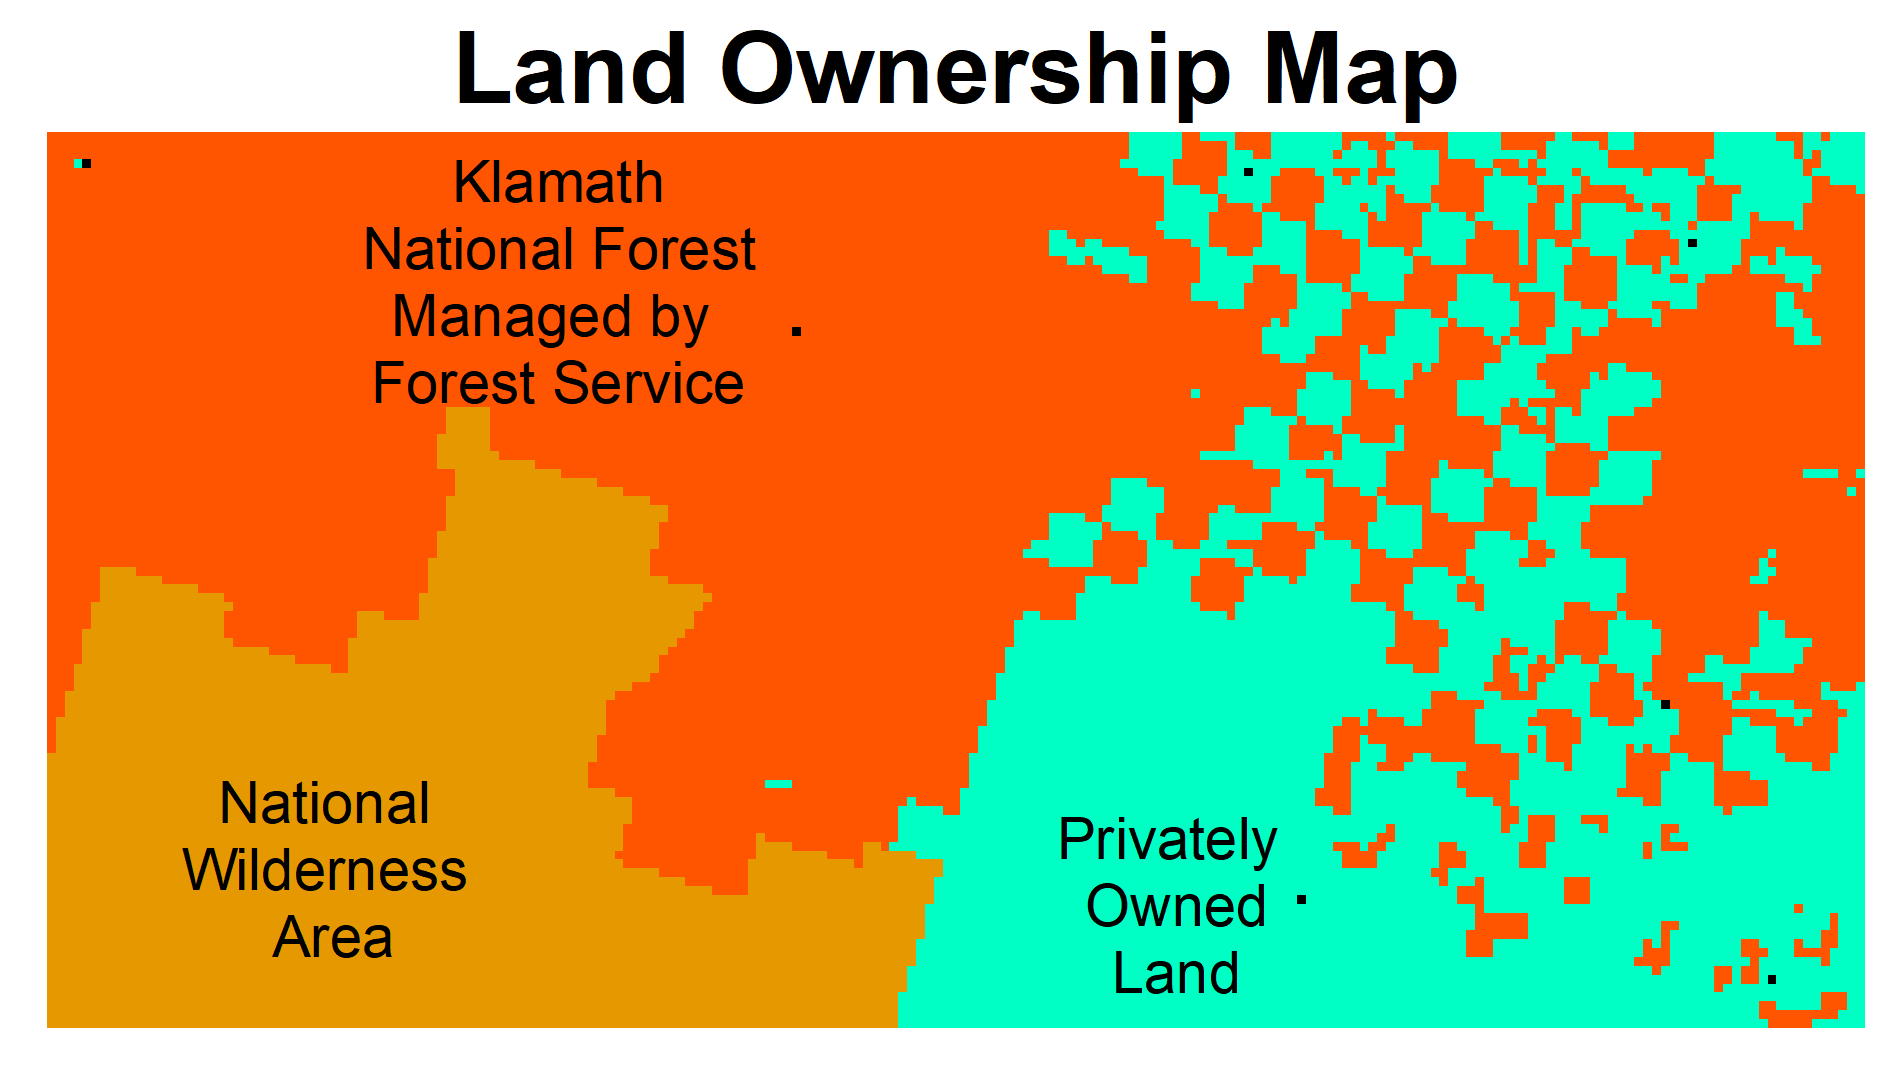
\includegraphics[width=\linewidth]{landOwnershipMap.png}
\end{subfigure}
\end{figure}

\end{frame}

\begin{frame}{Animated Fire History - A2 Climate \& LU+}

 %\animategraphics[loop,controls,width=\linewidth]{1.15}{./A2Climate_Fire_LU_GIF/A2fig}{1}{39}

\end{frame}

 \begin{frame}{Animated Fire History - Recent Trends \& LU+}
% \animategraphics[loop, controls, width=\textwidth]{1.15}{./NoClimate_Fire_LU_GIF/Nofig}{1}{39}
 \end{frame}



\begin{frame}{Mean Cut Return Interval}
\centering\includegraphics[width=.525\linewidth]{mean_cut_interval_2010-2050.png}
\end{frame}



\begin{frame}{Mean Fire Return Interval Map: By Land Owner}
\centering{
\includegraphics[width=.46\linewidth]{FSMask_mfri_2010-2100.jpg}
\hspace*{.75cm}
\includegraphics[width=.46\linewidth]{PrivMask_mfri_2010-2100.jpg}
}
\end{frame}


\begin{frame}{Mean Fire Return Interval Distribution: By Land Owner}
\centering{
\includegraphics[height=.6\linewidth]{DensityPlot_mfri_2010-2100.png}

}
\end{frame}
\end{comment}
\section{Putting the Pieces Together}
\subsection{}
\begin{frame}{Putting the Pieces Together in a GIF}
 \animategraphics[loop, controls, width=\textwidth, height=.5\textwidth]{1.15}{./NOGIF-Clean/RT}{1}{9}
\end{frame}


\begin{comment}
\begin{frame}{Implementing Human Response to Fire}




\end{frame}


\begin{frame}{Simulations}


\end{frame}


\section{Results}
\subsection{}
\begin{frame}{Affects of Climate}


\end{frame}


\begin{frame}{Affects of Human Response}

\end{frame}

\section{}

\begin{frame}{References}

\end{frame}



\appendix 
\begin{frame}[noframenumbering]{Additional Figures}

\end{frame}

\begin{frame}[noframenumbering]{Additional Figures 2}

\end{frame}
\end{comment}


\begin{comment}
\section{Extra Slides}
\subsection{}


\begin{frame}[noframenumbering]{CO2 Concentration}
\centering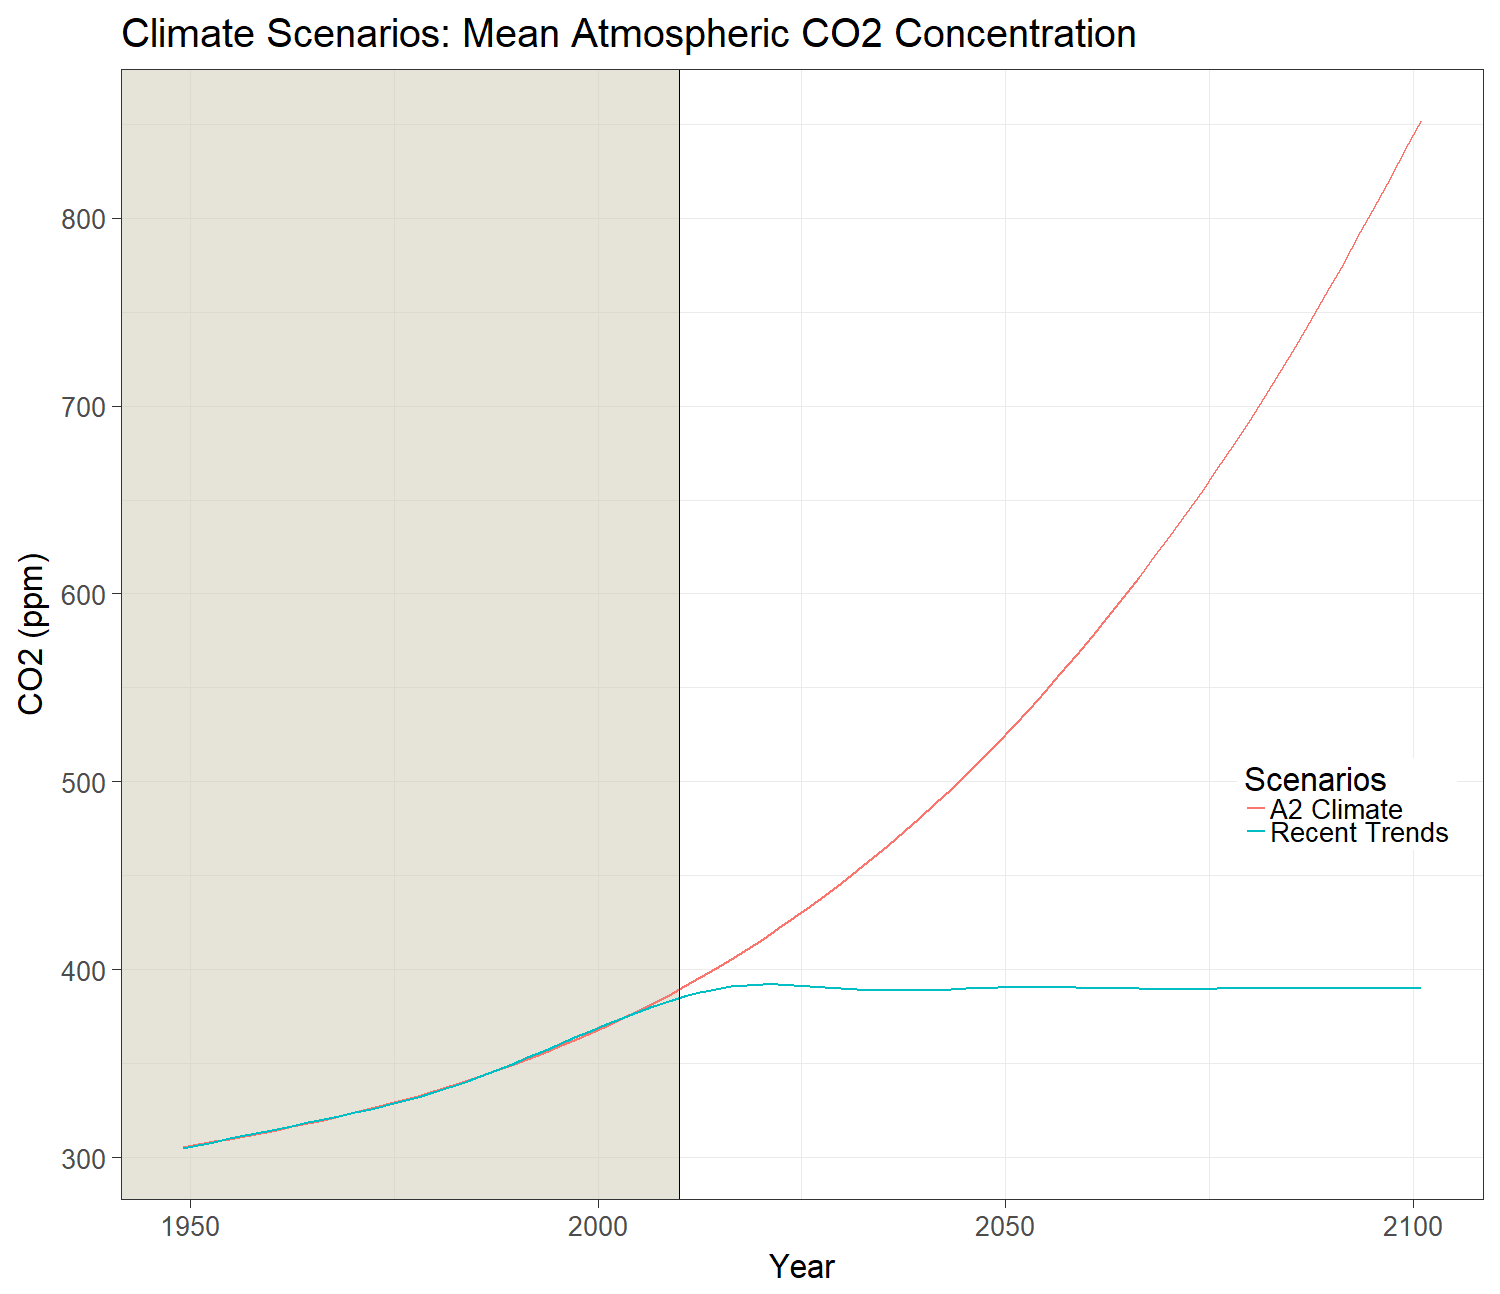
\includegraphics[width=.75\linewidth]{CO2_Concentration.png}
\end{frame}
\begin{comment}
\begin{frame}{Temperature by Ecoregion}
\centering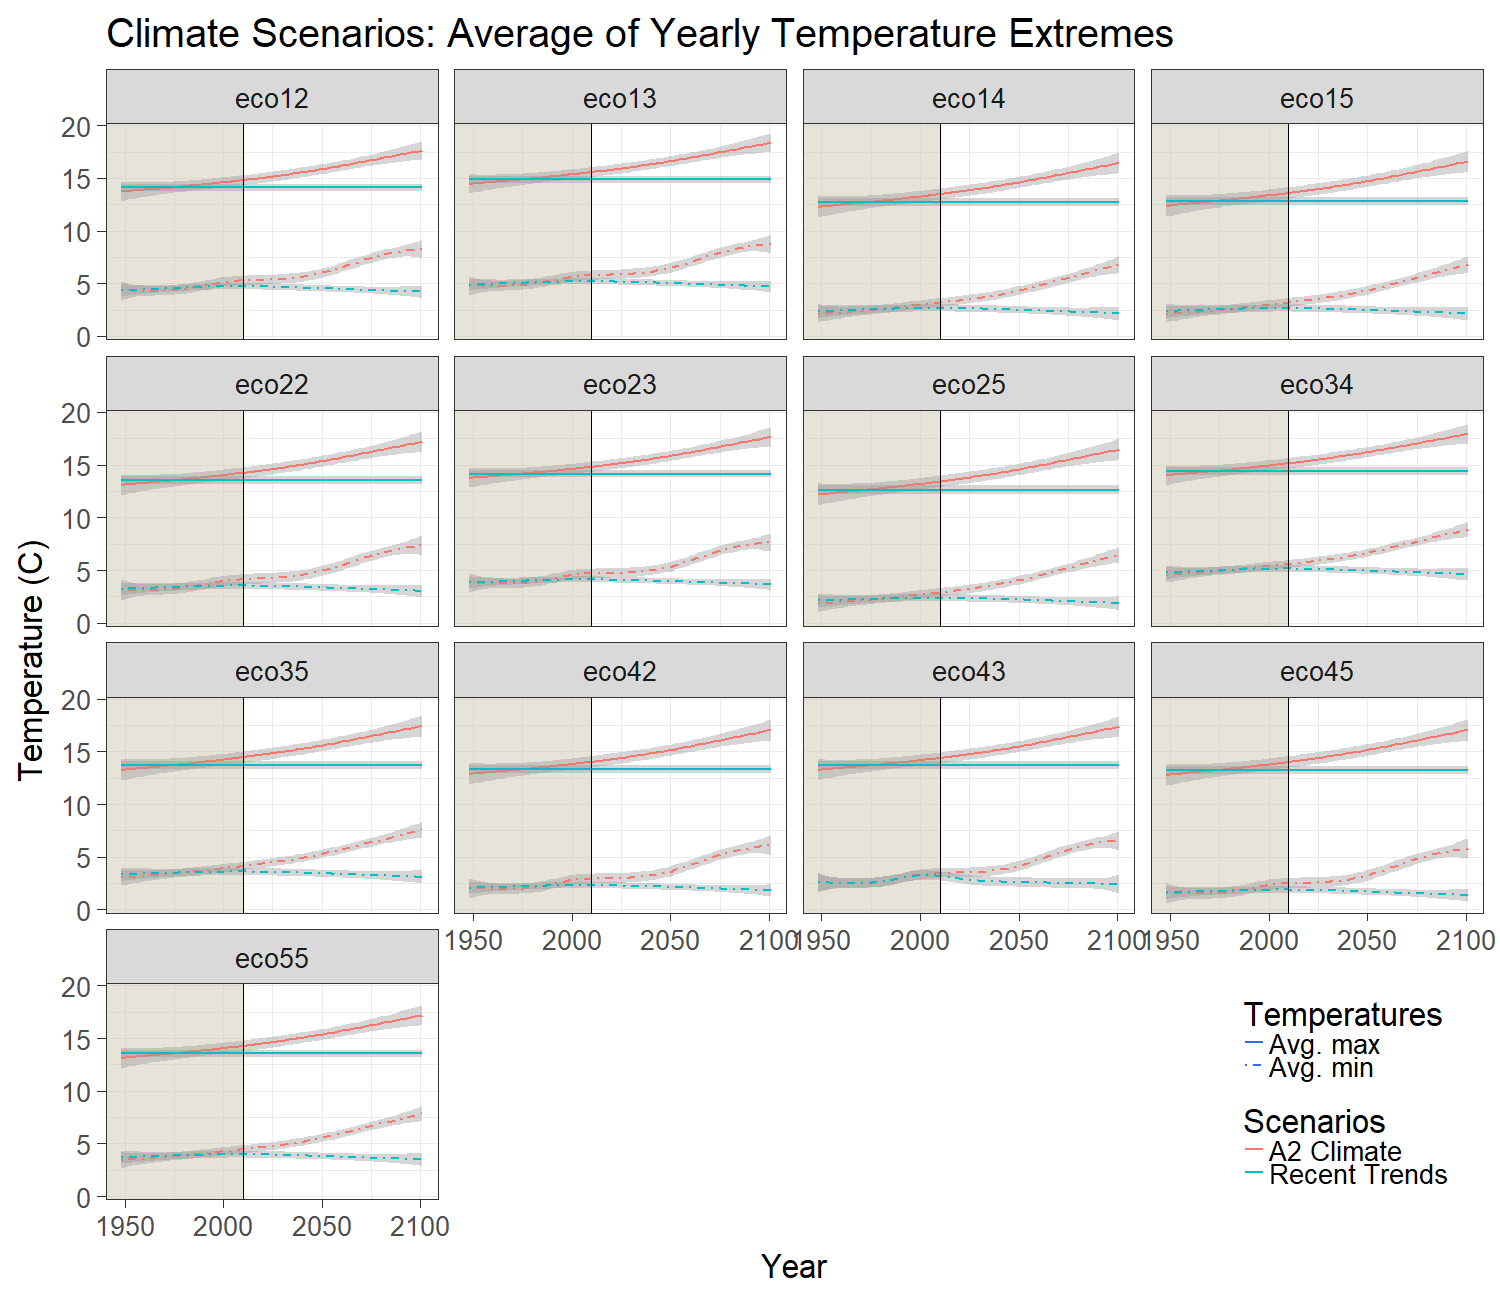
\includegraphics[width=.75\linewidth]{ECOREGION_Average_of_Yearly_Temperature_Extremes.png}

\end{frame}

\begin{frame}{Precipitation by Ecoregion}
\centering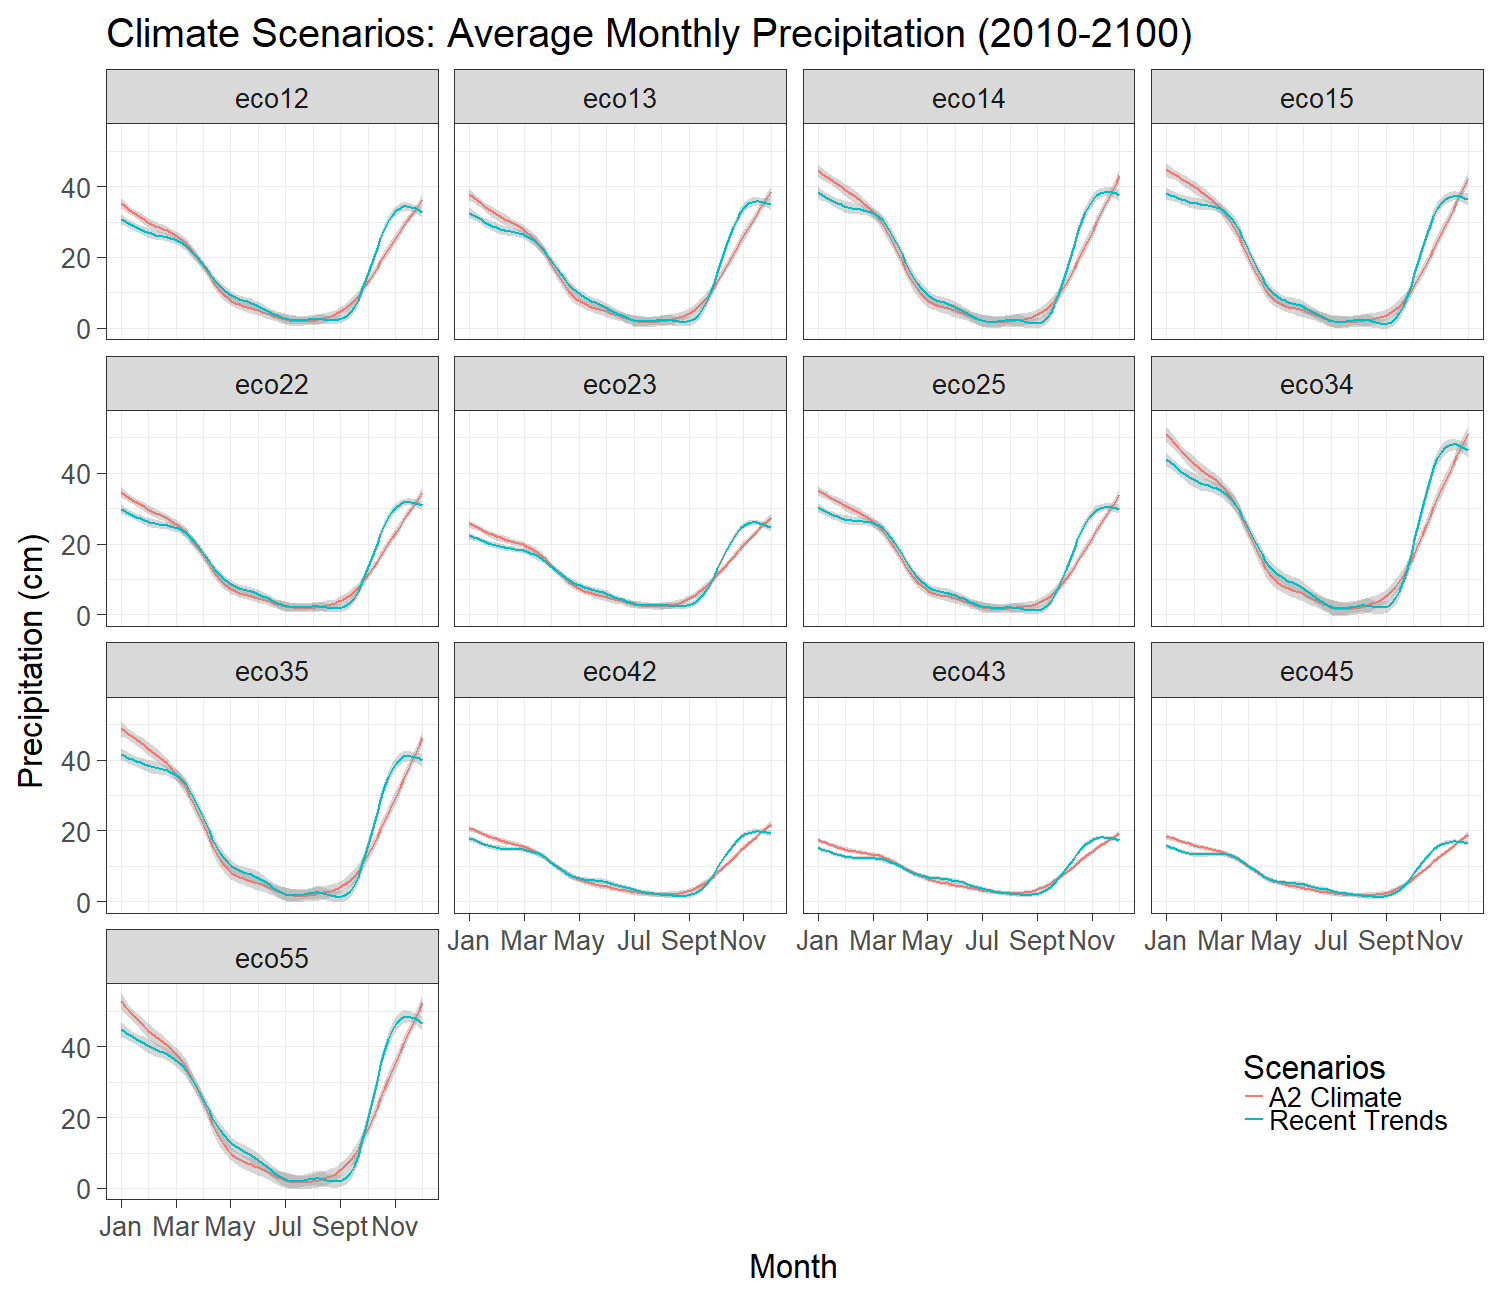
\includegraphics[width=.75\linewidth]{ECOREGION_Average_Monthly_Precipitation__2010-2100_.png}
\end{frame}
%\end{comment}

\begin{frame}[noframenumbering]{Shifts in Temperature Over Time}

\centering\includegraphics[width=.7\linewidth]{Temperature__2010-2100_.png}
\end{frame}

\begin{frame}[noframenumbering]{Shifts in Precipitation Over Time}
\centering\includegraphics[width=.7\linewidth]{Precipitation__2010-2100_.png}
\end{frame}



\begin{comment}
\begin{frame}[noframenumbering]{Woody Debris}
\centering\includegraphics[width=.75\linewidth]{woody_debris.png}
\end{frame}


\begin{frame}[noframenumbering]{FS owned land with Wilderness Area Map}
\centering\includegraphics[width=.9\linewidth]{fs_with_WA_mfri_2010-2050.png}
\end{frame}

\begin{frame}[noframenumbering]{FS owned land with Wilderness Area Histogram}
\centering\includegraphics[width=.725\linewidth]{fsowned_with_WA_mfri_histogram_2010-2050.png}
\end{frame}

\section{Extra Slides: 100 Year Climate}
\subsection{}

\begin{frame}[noframenumbering]{100 Year Climate Overall Trends}
%\centering\includegraphics[width=.725\linewidth]{fsowned_with_WA_mfri_histogram_2010-2050.png}
\end{frame}
\begin{frame}[noframenumbering]{Phases of Climate Precipitation}
%\centering\includegraphics[width=.725\linewidth]{fsowned_with_WA_mfri_histogram_2010-2050.png}
\end{frame}
\begin{frame}[noframenumbering]{Phases of Climate Temperature}
%\centering\includegraphics[width=.725\linewidth]{fsowned_with_WA_mfri_histogram_2010-2050.png}
\end{frame}

\begin{frame}[noframenumbering]{100 Year Temperature by Ecoregion}
%\centering\includegraphics[width=.725\linewidth]{fsowned_with_WA_mfri_histogram_2010-2050.png}
\end{frame}
\begin{frame}[noframenumbering]{100 Year Precipitation by Ecoregion}
%\centering\includegraphics[width=.725\linewidth]{fsowned_with_WA_mfri_histogram_2010-2050.png}
\end{frame}
\end{comment}


\begin{frame}{Total Aboveground Biomass}
\centering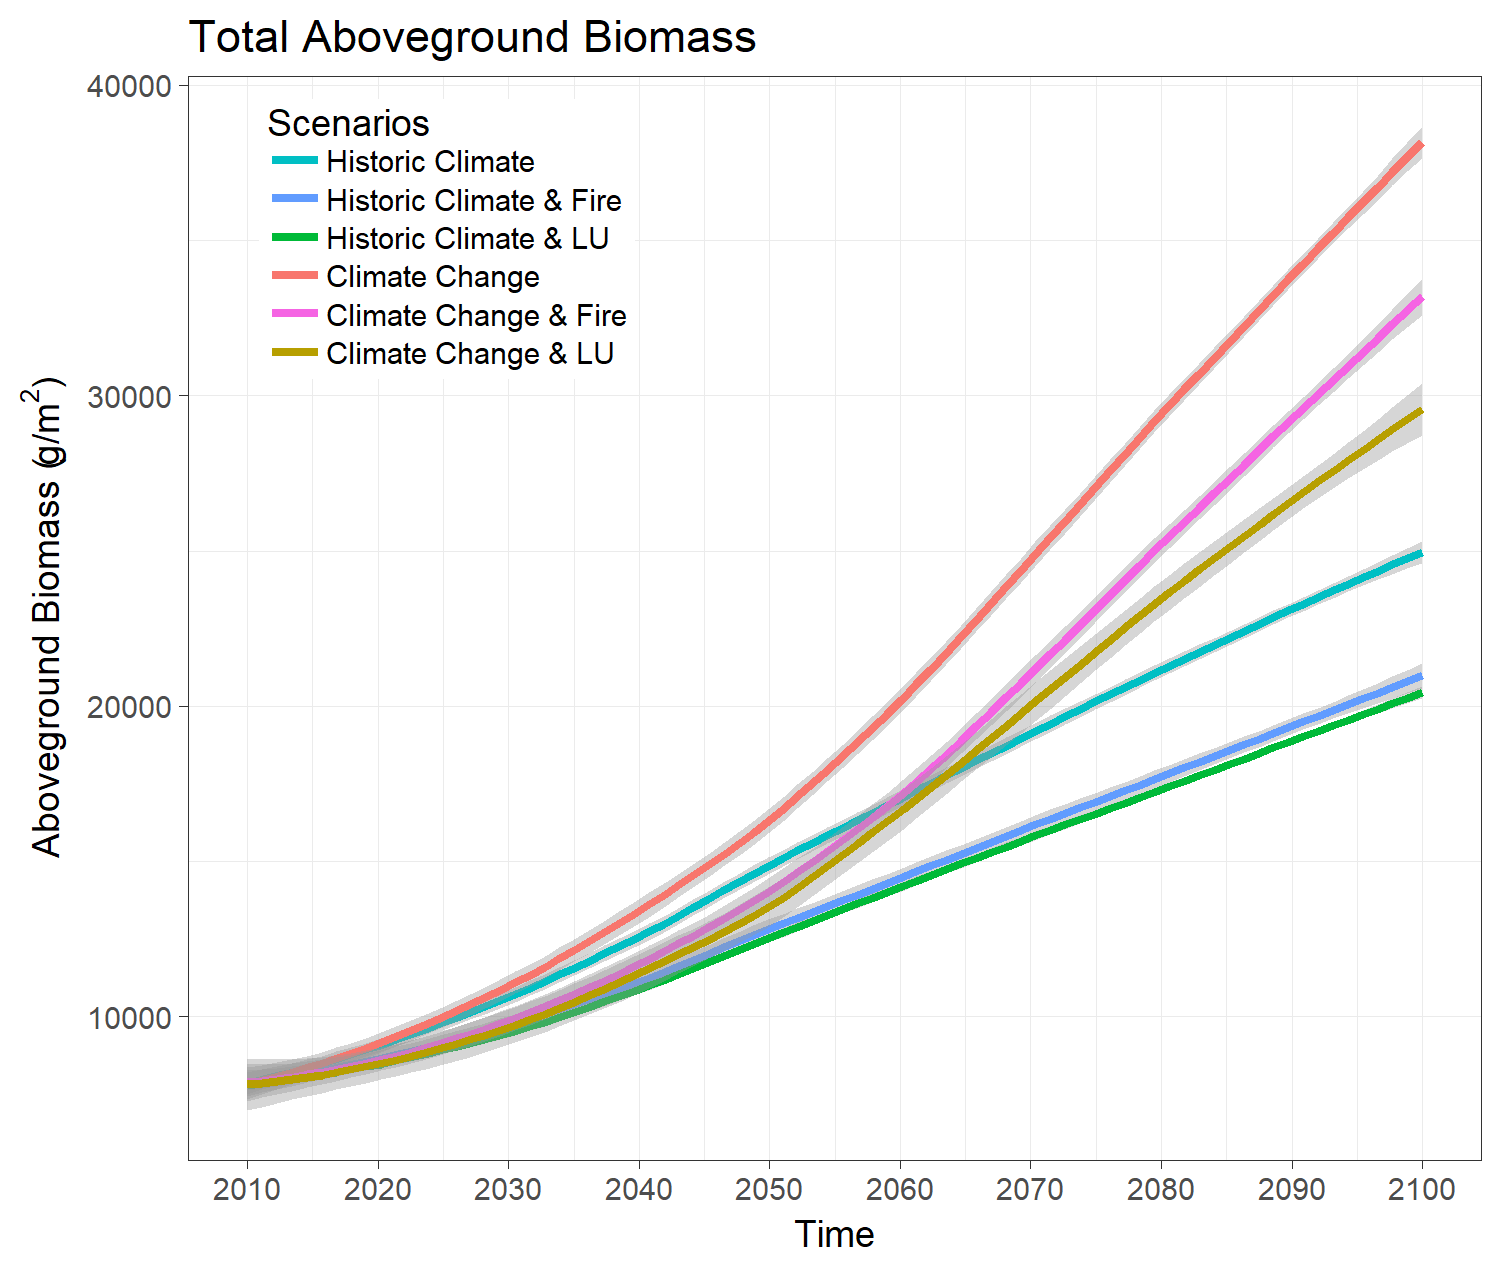
\includegraphics[width=.75\linewidth]{AGB_legend_fix.png}
\end{frame}

\begin{frame}{The Need for Replicates}
\centering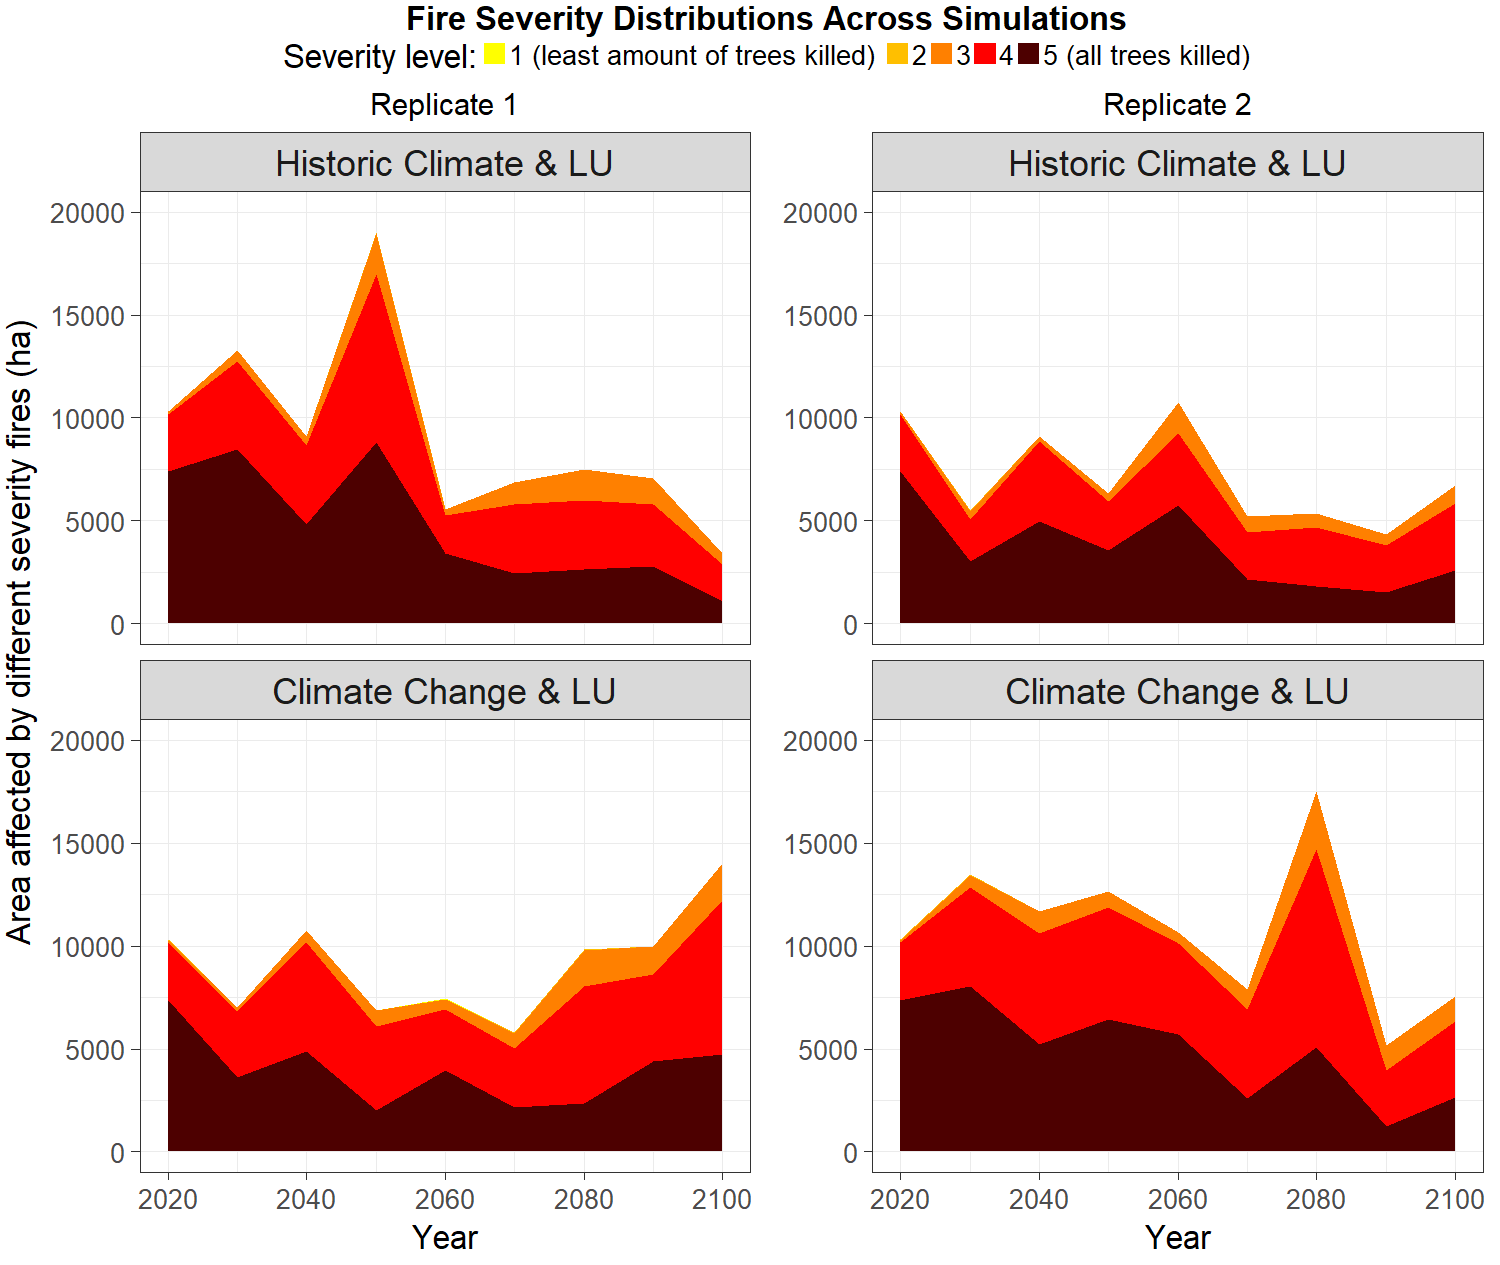
\includegraphics[width=.725\linewidth]{firedisrealFINAL.png}

\end{frame}

\appendix
\begin{frame}[noframenumbering]
\centering\Huge{\color{FuchsiaDark} Questions?}\\[1cm]
\end{frame}

\end{document}


